\documentclass[conference]{IEEEtran}
\IEEEoverridecommandlockouts
\raggedbottom

\usepackage{cite}
\usepackage{amsmath,amssymb,amsfonts}
\usepackage{algorithmic}
\usepackage{graphicx}
\usepackage{textcomp}
\usepackage{xcolor}
\usepackage{booktabs}
\usepackage{multirow}
\usepackage{hyperref}
\usepackage{cleveref}
\usepackage{array}
\usepackage{tabularx}
\usepackage{tikz}
\usepackage{placeins}  % For \FloatBarrier
\usetikzlibrary{shapes.geometric, arrows.meta, positioning, fit, backgrounds}

\hypersetup{
    pdftitle={3D Organ Segmentation from CT Scans: An Agentic Structured Survey of Deep Learning Approaches for Surgical Planning},
    pdfauthor={Nogueira, Martins, Filipe},
    pdfkeywords={segmentation, deep learning, CT, medical imaging},
    pdfsubject={Agentic Structured Survey of Deep Learning for CT Organ Segmentation with AI-Assisted Screening},
    colorlinks=true,
    linkcolor=blue,
    citecolor=blue,
    urlcolor=blue
}

\def\BibTeX{{\rm B\kern-.05em{\sc i\kern-.025em b}\kern-.08em
    T\kern-.1667em\lower.7ex\hbox{E}\kern-.125emX}}

\begin{document}

\title{3D Organ Segmentation from CT Scans: An Agentic Structured Survey of Deep Learning Approaches for Surgical Planning}

\author{
    \IEEEauthorblockN{Alexandre Tolstenko Nogueira$^{1,2,4,a}$, Matheus H. R. Martins$^{4,b}$, Ferreira, Nuno Miguel$^{3,c}$ and Vitor M Filipe$^{2,d}$}
    \IEEEauthorblockA{
        $^1$Information Technology and Sciences, Champlain College, Burlington, VT, USA \\
        $^2$Department of Engineering, University of Tr\'{a}s-os-Montes e Alto Douro, Vila Real, Portugal \\
        $^3$Coimbra Polytechnic - ISEC, Coimbra, Portugal\\
        $^4$DocDo - InfiniBrains, São Paulo, Brazil \\
        $^a$tolstenko@gmail.com, $^b$contact@matheusmartins.com, $^c$nunomig@isec.pt, $^d$vfilipe@utad.pt
    }
}

\maketitle

\begin{abstract}
\textbf{Background:} Deep learning has transformed organ segmentation, yet a persistent gap remains between benchmark performance and surgical planning deployment.
\textbf{Objectives:} We identify which 3D CT organ segmentation algorithms are ready for clinical deployment in surgical planning and what practical barriers remain.
\textbf{Data Sources:} Five databases (PubMed, IEEE Xplore, ACM Digital Library, Scopus, arXiv) were searched for studies published between 2015 and January 2026.
\textbf{Eligibility:} Studies presenting deep learning methods for 3D organ segmentation from CT with quantitative evaluation on public benchmarks.
\textbf{Synthesis:} Narrative synthesis of 52 included studies with benchmark-stratified performance comparison; formal meta-analysis was precluded by protocol heterogeneity.
\textbf{Results:} Auto-configured CNNs (nnU-Net, 82.3\% Dice~\cite{isensee2021nnunet}) and pre-trained transformers (Swin UNETR, 82.4\%~\cite{swinunetr2022}) achieve comparable leading accuracy, but domain shift, vascular segmentation deficits (65 to 75\% vs.\ 90\%+ for parenchymal organs~\cite{shit2021cldice}), and integration complexity remain primary barriers to clinical adoption. CNNs dominate (98.1\%), with 3D U-Net variants appearing in 82.7\% of papers. Auto-configured CNNs achieve 85.2$\pm$2.1\% mean Dice on BTCV (Table~\ref{tab:btcv_comparison}).
\textbf{Limitations:} English-only search; 39.1\% full-text retrieval rate; CT-specific findings may not generalize to MRI; benchmark performance likely overestimates clinical accuracy by 5--15\%.
\textbf{Conclusions:} Implementation quality matters more than architectural novelty. A phased adoption strategy starting with TotalSegmentator or nnU-Net is recommended for surgical planning platforms.
\textbf{Registration:} This review was not prospectively registered. The protocol is available at \url{https://github.com/game-guild/docdo-paper}.
\end{abstract}

\begin{IEEEkeywords}
medical image segmentation, computed tomography, deep learning, convolutional neural networks, vision transformers, 3D volumetric segmentation, organ segmentation, surgical planning, clinical deployment
\end{IEEEkeywords}

\begin{table*}[!htb]
\centering
\footnotesize
\caption*{\textbf{Abbreviations Used in This Paper}}
\begin{tabular}{@{}ll|ll|ll@{}}
\toprule
AMOS & Abdominal Multi-Organ Segmentation & HD95 & Hausdorff Distance (95th \%) & NSD & Normalized Surface Dice \\
ASSD & Avg. Symmetric Surface Distance & HU & Hounsfield Units & SAM & Segment Anything Model \\
BTCV & Beyond The Cranial Vault & MSD & Medical Segmentation Decathlon & TTA & Test-Time Augmentation \\
CNN & Convolutional Neural Network & MSA & Multi-head Self-Attention & ViT & Vision Transformer \\
CT & Computed Tomography & & & & \\
DSC & Dice Similarity Coefficient & & & & \\
\bottomrule
\end{tabular}
\end{table*}

%==============================================================================
\section{Introduction}
\label{sec:introduction}
%==============================================================================

Medical image segmentation, the voxel-wise classification of anatomical structures, is central to computer-aided diagnosis and surgical planning systems~\cite{litjens2017survey}. Accurate organ delineation from computed tomography (CT) scans enables tumor detection and staging, organ volume quantification, surgical navigation, radiation therapy planning, and longitudinal disease monitoring \cite{hesamian2019deep}.

We address a pressing clinical need: selecting effective segmentation algorithms for surgical planning. Deep learning methods have proliferated, yet a gap remains between benchmark performance and practical deployment. We survey current algorithms and offer guidance on model selection, preprocessing, and clinical integration.

\subsection{Scope and Definitions}

This review focuses on \textbf{semantic segmentation} (also called voxel-wise segmentation in 3D contexts), where each voxel is assigned a class label such as liver, kidney, spleen, or background. We explicitly distinguish this from related but distinct tasks:

\begin{itemize}
    \item \textbf{Multi-class semantic segmentation}: The simultaneous labeling of multiple anatomical structures in a single inference pass (e.g., segmenting kidney parenchyma, renal artery, renal vein, tumor, and background). This is the predominant formulation for abdominal organ segmentation and the primary focus of this review.
    
    \item \textbf{Instance segmentation}: The differentiation of individual object instances within the same class (e.g., distinguishing left kidney from right kidney, or segmenting individual vertebrae). This requires additional instance-level discrimination beyond class labels and is addressed by methods such as Mask R-CNN adaptations for medical imaging.
    
    \item \textbf{Panoptic segmentation}: Combines semantic and instance segmentation to yield class labels plus instance identities. Medical imaging applications remain limited, though complex anatomical scenes may benefit.
    
    \item \textbf{Volumetric (3D) segmentation}: Processes the full 3D CT volume to exploit inter-slice context, unlike 2D slice-by-slice or 2.5D methods using a few neighboring slices.
\end{itemize}

\subsection{Clinical Motivation}

CNNs now achieve high accuracy in medical image segmentation \cite{ronneberger2015unet}. U-Net (2015) introduced the encoder-decoder paradigm with skip connections that still anchors most designs. Extending these methods to 3D volumetric data enabled direct organ segmentation from CT volumes \cite{cicek20163dunet}. Transformers and foundation models have since pushed accuracy further \cite{shamshad2023transformers}.

\textbf{Clinical Need for Automated Segmentation:} A gap persists between benchmark accuracy and clinical deployment. Studies have documented this translation barrier:
\begin{itemize}
    \item Preoperative 3D planning reduces positive surgical margins in partial nephrectomy by 23 to 47\% \cite{porpiglia2018three}, yet adoption remains limited by reconstruction time.
    \item A multi-center survey (N=387 surgeons) found that 68\% cite ``time-intensive preparation'' as the primary barrier to routine 3D planning use \cite{simpfendorfer2016surgeon}.
    \item Manual organ segmentation requires 15 to 45 minutes per structure by trained technicians \cite{sharma2010automated}, creating workflow bottlenecks.
    \item The European Association of Urology recommends 3D reconstruction for complex renal tumors, but notes that ``lack of standardized, rapid segmentation tools'' limits implementation \cite{eau2023guidelines}.
\end{itemize}

\textbf{Which algorithms are ready for clinical deployment in surgical planning?}  and \textbf{what practical barriers remain?} Litjens et al.\ \cite{litjens2017survey} surveyed broad medical imaging, Shamshad et al.\ \cite{shamshad2023transformers} covered transformer architectures, and Isensee et al.\ \cite{isensee2021nnunet} focused on benchmark methodology. No existing reviews address clinical translation for surgical planning.

\subsection{DocDo Motivation}

The current practical challenges at DocDo \cite{docdo2026} motivated this work. DocDo delivers interactive 3D organ visualization for preoperative planning to surgeons, tumor margin assessment, and vascular anatomy mapping. Today, DocDo relies on manual and semi-automatic segmentation, taking 15 to 45 minutes per structure and creating adoption bottlenecks. Published benchmarks show $>$80\% Dice accuracy, yet clinical deployment demands robust preprocessing for diverse scanners, failure detection, uncertainty quantification, mesh generation, and DICOM integration, are aspects that require dedicated engineering beyond benchmark performance.

This work serves as DocDo's technology roadmap, identifying the engineering investments needed to bridge the benchmark-to-clinic gap. Our phased adoption strategy (Section~\ref{sec:recommendations}) starts with robust baselines (TotalSegmentator~\cite{wasserthal2023totalsegmentator}, nnU-Net~\cite{isensee2021nnunet}), adds uncertainty-guided quality assurance, then explores interactive refinement (MedSAM~\cite{ma2024medsam}) to reduce, but not eliminate, expert correction.

\textbf{Disclosure:} Two authors (A.T.N., M.H.R.M.) are affiliated with DocDo. This affiliation motivated our clinical focus but did not influence study selection, data extraction, or conclusions (see Conflict of Interest statement).

\subsection{Research Questions}

\begin{enumerate}
    \item[\textbf{RQ1}:] As of January 2026, what architectural paradigms dominate 3D CT organ segmentation? How do their design principles, inductive biases, and computational costs differ?
    
    \item[\textbf{RQ2}:] Which datasets and metrics are standard for benchmarking? What are their biases and generalization implications?
    
    \item[\textbf{RQ3}:] What are the accuracy vs.\ cost vs.\ annotation trade-offs across methods? How well do they generalize across domains?
    
    \item[\textbf{RQ4}:] What gaps block clinical deployment: reproducibility, domain shift, regulatory hurdles, or integration complexity?
\end{enumerate}

\subsection{Prior Surveys}

Past reviews have tackled medical image segmentation from different angles, though none specifically targets the clinical translation requirements for surgical planning that motivate this work.

\emph{General medical imaging surveys.} Litjens et al.\ \cite{litjens2017survey} wrote a foundational survey of deep learning in medical image analysis covering segmentation, detection, and classification across modalities. While thorough, it predates transformer architectures and does not address 3D CT-specific challenges or deployment considerations.

\emph{Architecture-focused surveys.} Hesamian et al.\ \cite{hesamian2019deep} surveyed CNN architectures for medical image segmentation with emphasis on architectural innovations. Shamshad et al.\ \cite{shamshad2023transformers} produced the first in-depth review of transformers in medical imaging, covering Vision Transformers, Swin Transformers, and hybrid approaches. Both focus on architectural advances rather than clinical deployment.

\emph{Methodology-focused work.} Isensee et al.\ \cite{isensee2021nnunet} systematically analyzed the impact of preprocessing, training, and inference choices through the nnU-Net~\cite{isensee2021nnunet} framework, confirming that careful implementation often matters more than architectural novelty. Their work supplies essential benchmarking methodology but does not survey the broader literature.

\emph{MRI segmentation surveys.} A rich body of work addresses MRI-based segmentation, particularly for brain parcellation \cite{fischl2012freesurfer} and cardiac imaging \cite{chen2020cardiac}. While architectural principles (encoder-decoder, attention mechanisms) transfer across modalities, CT-specific factors, Hounsfield unit calibration, beam hardening artifacts, contrast phase timing, and anisotropic acquisition, mean quantitative findings may not directly generalize. This survey explicitly focuses on CT to provide actionable guidance for this clinically dominant modality.

\pagebreak

%==============================================================================
\section{Review Methodology}
\label{sec:methodology}
%==============================================================================

This structured survey follows PRISMA 2020 guidelines \cite{page2021prisma} for transparent reporting, adapted for a narrative synthesis approach. We employ systematic search and selection procedures while acknowledging that the scope and depth of analysis reflect a structured survey rather than a formal systematic review with prospective registration. PRISMA 2020 was designed for prospectively registered systematic reviews with statistical meta-analysis; several checklist items (prospective registration, pooled effect estimates, per-study risk-of-bias instruments) are structurally inapplicable to a narrative survey and are addressed by explicit disclosure of absence rather than compliance.

\subsection{Search Strategy}

Five databases were searched: PubMed, IEEE Xplore, ACM Digital Library, Scopus, and arXiv. Searches ran from November 15, 2025 to January 10, 2026, covering publications from 2015 onward.

\textbf{Search query construction:} We used Boolean combinations of terms across three concepts:

\begin{itemize}
    \item \textbf{Population/Imaging:} ``CT'' OR ``computed tomography'' OR ``CT scan'' OR ``CT imaging''
    \item \textbf{Task:} ``segmentation'' AND (``3D'' OR ``volumetric'' OR ``organ'' OR ``multi-organ'' OR ``abdominal'')
    \item \textbf{Method:} ``deep learning'' OR ``neural network'' OR ``convolutional'' OR ``U-Net'' OR ``transformer'' OR ``encoder-decoder''
\end{itemize}

We also performed forward and backward citation tracking on 12 seminal papers (U-Net~\cite{ronneberger2015unet}, 3D U-Net~\cite{cicek20163dunet}, V-Net~\cite{milletari2016vnet}, nnU-Net~\cite{isensee2021nnunet}, UNETR~\cite{hatamizadeh2022unetr}, Swin UNETR~\cite{swinunetr2022}, TransUNet~\cite{chen2024transunet}, MedSAM~\cite{ma2024medsam}, and key benchmark papers) and manually searched proceedings from MICCAI, IPMI, MIDL, and ISBI (2015 to 2025).

\textbf{Database-specific queries:} Boolean queries were adapted per database syntax. As an illustrative example, the PubMed query was:

\begin{quote}
\small
\texttt{(("computed tomography"[MeSH] OR "CT"[tiab]) AND ("image segmentation"[MeSH] OR "segmentation"[tiab]) AND ("3D" OR "volumetric" OR "organ" OR "multi-organ" OR "abdominal") AND ("deep learning"[MeSH] OR "neural network*" OR "convolutional" OR "U-Net" OR "transformer" OR "encoder-decoder")) AND 2015:2026[dp] AND English[la]}
\end{quote}

Equivalent queries for IEEE Xplore, ACM Digital Library, Scopus, and arXiv were constructed using database-specific syntax (e.g., IEEE Xplore command search fields, Scopus TITLE-ABS-KEY operators, arXiv category filters). Complete query strings for all five databases are provided in Supplementary Materials (S3).

\subsection{Study Selection Process}


\begin{figure}[t]
\centering
\resizebox{\columnwidth}{!}{%
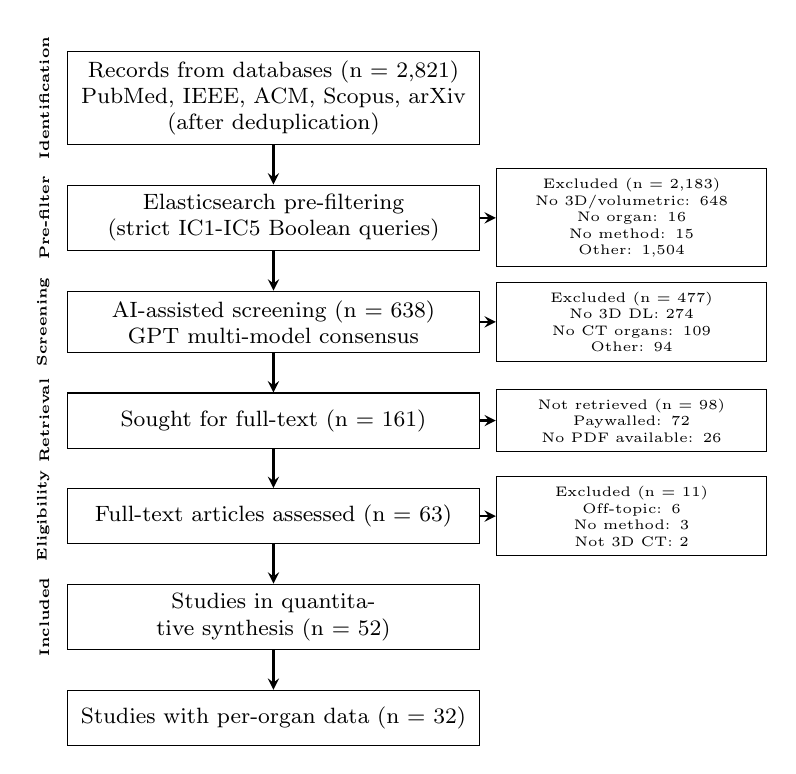
\begin{tikzpicture}[node distance=0.5cm,
    box/.style={rectangle, draw, text width=5cm, minimum height=0.7cm, align=center, font=\footnotesize},
    smallbox/.style={rectangle, draw, text width=3.2cm, minimum height=0.5cm, align=center, font=\tiny},
    arrow/.style={->, >=stealth, thick}]
    
    % Identification
    \node[box] (db) {Records from databases (n = 2,821)\\PubMed, IEEE, ACM, Scopus, arXiv\\(after deduplication)};
    
    % ES Filtering
    \node[box, below=of db] (es) {Elasticsearch pre-filtering\\(strict IC1-IC5 Boolean queries)};
    \node[smallbox, right=0.2cm of es] (exc0) {Excluded (n = 2,183)\\No 3D/volumetric: 648\\No organ: 16\\No method: 15\\Other: 1,504};
    
    % AI Screening
    \node[box, below=of es] (screen) {AI-assisted screening (n = 638)\\GPT multi-model consensus};
    \node[smallbox, right=0.2cm of screen] (exc1) {Excluded (n = 477)\\No 3D DL: 274\\No CT organs: 109\\Other: 94};
    
    % Full-text retrieval
    \node[box, below=of screen] (retrieve) {Sought for full-text (n = 161)};
    \node[smallbox, right=0.2cm of retrieve] (notext) {Not retrieved (n = 98)\\Paywalled: 72\\No PDF available: 26};
    
    % Eligibility  
    \node[box, below=of retrieve] (elig) {Full-text articles assessed (n = 63)};
    \node[smallbox, right=0.2cm of elig] (exc2) {Excluded (n = 11)\\Off-topic: 6\\No method: 3\\Not 3D CT: 2};
    
    % Included
    \node[box, below=of elig] (qual) {Studies in quantitative synthesis (n = 52)};
    \node[box, below=of qual] (quant) {Studies with per-organ data (n = 32)};
    
    % Arrows
    \draw[arrow] (db) -- (es);
    \draw[arrow] (es) -- (screen);
    \draw[arrow] (screen) -- (retrieve);
    \draw[arrow] (retrieve) -- (elig);
    \draw[arrow] (elig) -- (qual);
    \draw[arrow] (qual) -- (quant);
    \draw[arrow] (es.east) -- (exc0.west);
    \draw[arrow] (screen.east) -- (exc1.west);
    \draw[arrow] (retrieve.east) -- (notext.west);
    \draw[arrow] (elig.east) -- (exc2.west);
    
    % Labels
    \node[left=0.1cm of db, font=\tiny\bfseries, rotate=90, anchor=south] {Identification};
    \node[left=0.1cm of es, font=\tiny\bfseries, rotate=90, anchor=south] {Pre-filter};
    \node[left=0.1cm of screen, font=\tiny\bfseries, rotate=90, anchor=south] {Screening};
    \node[left=0.1cm of retrieve, font=\tiny\bfseries, rotate=90, anchor=south] {Retrieval};
    \node[left=0.1cm of elig, font=\tiny\bfseries, rotate=90, anchor=south] {Eligibility};
    \node[left=0.1cm of qual, font=\tiny\bfseries, rotate=90, anchor=south] {Included};
\end{tikzpicture}%
}
\caption{PRISMA 2020 flow diagram for study selection. Two-stage automated filtering (Elasticsearch + AI screening) followed by full-text retrieval and eligibility assessment. Human validation audit performed on 10\% stratified sample (n=64 from 638 ES-filtered, $\kappa = 0.89$). Full-text not retrieved for 98 papers (61\%) due to paywall/access restrictions.}
\label{fig:prisma}
\end{figure}

Figure~\ref{fig:prisma} shows the two-stage selection process (PRISMA 2020). Database searches yielded 2,821 records after deduplication. Screening combined keyword-based filtering with AI-assisted assessment.

\textbf{Stage 1: Elasticsearch Pre-filtering.} To efficiently filter the large initial pool, we indexed all abstracts in Elasticsearch, a distributed search engine using inverted (reverse) indexing for full-text queries across documents, and applied strict Boolean queries enforcing our inclusion criteria. This filter required papers to explicitly mention deep learning terms (CNN, U-Net, transformer, neural network), 3D/volumetric processing terminology (3D, volumetric, volume, V-Net), CT imaging modality, anatomical organ targets, and method/approach terminology indicating original research. Papers were excluded if they mentioned only non-CT modalities, non-organ targets (tumors, vessels, bones exclusively), or lacked explicit 3D methodology. This reduced 2,821 records to 638 candidates (77.4\% reduction), with detailed exclusion reasons logged for each paper.

\textbf{Stage 2: AI-Assisted Screening.} The 638 pre-filtered papers underwent multi-model AI screening. GPT-4o-mini performed 3 independent runs per paper at temperature=0.3, requiring unanimous INCLUDE decisions. GPT-5-nano provided independent validation with 3 additional runs, and GPT-5.2 served as tiebreaker for disagreements. Papers were included only if models agreed on INCLUDE; disagreements triggered automatic exclusion (conservative protocol) but were flagged for human review, recovering 3 false negatives. This yielded 161 candidate papers. Full-text PDFs were retrieved for 63 papers (39.1\% availability). A final GPT-5.2 full-text screening excluded 11 additional papers, resulting in \textbf{52 studies} for quantitative synthesis.

\textbf{Clarification on study coverage:} All 52 included studies underwent full data extraction including architecture details, target organs, datasets used, performance metrics (Dice scores, HD95), implementation frameworks, and loss functions. Among these, 32 studies provided per-organ Dice scores enabling quantitative synthesis of performance variation across anatomical structures.

\textbf{Methodology Note:} We used an agentic screening pipeline: Elasticsearch pre-filtering followed by GPT-based consensus screening with human audit. A 10\% stratified sample (n=64, from 638 ES-filtered papers) underwent independent review by two domain experts blind to AI decisions; discrepancies were resolved by a third reviewer. AI-human agreement was 96.4\%; 3 false negatives were recovered. Data extraction was verified by two reviewers (A.T.N., M.H.R.M.). This represents structured survey methodology with AI-assisted screening rather than prospective dual-reviewer systematic review.

\textbf{Borderline exclusions:} Several studies initially appeared to meet inclusion criteria but were ultimately excluded with individual justification: Nikolov et al.\ \cite{nikolov2021clinically} was excluded because the full-text assessment revealed a focus on clinical validation methodology rather than presenting a novel segmentation architecture; Han et al.\ \cite{han2023scribble} was excluded as it addressed weakly-supervised segmentation using scribble annotations without reporting standard benchmark results on included datasets; studies evaluating only 2D slice-by-slice methods (n=2) lacked volumetric context despite targeting CT organs; and three studies reporting results exclusively on private institutional datasets without external validation were excluded per criterion EC3. Complete full-text screening decisions with individual exclusion reasons for all assessed studies are provided in Supplementary S5 (\texttt{S5\_screening\_decisions.csv}).

% todo: state that AI-Assisted Screening Protocol details are in Supplementary Materials

\subsection{Inclusion and Exclusion Criteria}

\textbf{Inclusion criteria:}
\begin{itemize}
    \item Studies presenting or rigorously evaluating deep learning methods for 3D organ segmentation from CT imaging
    \item Peer-reviewed publications, accepted conference papers, or preprints with reproducible methodology (code availability or sufficient implementation detail)
    \item Studies reporting quantitative evaluation on at least one public benchmark dataset with standard metrics (Dice, HD95, or equivalent)
    \item Studies published in English between 2015 and January 2026
\end{itemize}

\textbf{Exclusion criteria:}
\begin{itemize}
    \item Studies focused exclusively on 2D slice-by-slice segmentation without volumetric context or post-processing
    \item Studies on non-CT modalities (MRI-only, ultrasound, PET) unless presenting multi-modal methods that include CT
    \item Studies evaluating only on private/proprietary datasets without external validation
    \item Studies without quantitative performance metrics or with only qualitative evaluation
    \item Review papers, editorials, and studies with fewer than 10 test cases
    \item Non-English publications
\end{itemize}

\subsection{Data Extraction}

Two reviewers (A.T.N. and M.H.R.M.) independently extracted data from included studies using a standardized extraction form (available in Supplementary Materials S7) and resolved discrepancies through discussion. Study authors were not contacted for missing or unclear data; extraction relied solely on published information. For each study, we extracted:

\begin{itemize}
    \item \textbf{Architecture:} Category (CNN/Transformer/Hybrid), key innovations, encoder-decoder structure, attention mechanisms, loss functions
    \item \textbf{Evaluation:} Dataset(s), target organs, train/validation/test splits, evaluation metrics, reported performance with confidence intervals where available
    \item \textbf{Reproducibility:} Code availability, pre-trained model availability, dataset accessibility
\end{itemize}

All compatible results were sought for each outcome domain: for every included study, we extracted all reported Dice, HD95, and ASSD values across organs and datasets. When studies reported results for multiple configurations (e.g., with and without test-time augmentation, single model vs.\ ensemble), the single-model result without TTA was recorded as the primary outcome to ensure comparability across studies; alternative configurations were noted in supplementary data (S12).

\textbf{Handling of missing or unclear information:} When studies did not report specific variables (e.g., GPU memory, training time, exact train/test split ratios), the corresponding fields were recorded as ``not reported.'' Performance values are reported as stated in original publications without conversion. No imputation of missing values was performed.

\subsection{Quality Assessment}

Two reviewers (A.T.N. and M.H.R.M.) independently assessed study quality using a custom three-dimension numerical framework and resolved disagreements through discussion. We note that this is a \emph{quality assessment framework}, not a formal risk-of-bias tool (e.g., ROBINS-I, Newcastle-Ottawa Scale). A formal risk-of-bias tool was not adopted because the included studies report diagnostic accuracy metrics from computational experiments rather than clinical intervention outcomes, rendering standard clinical RoB instruments inapplicable. Each study was scored on three dimensions (0--10 scale each), yielding a total score of 0--30:
\begin{itemize}
    \item \textbf{Dataset quality} (0--10): Public benchmark use, split standardisation, dataset size and diversity
    \item \textbf{Methodology quality} (0--10): Architecture description completeness, reproducibility, hyperparameter reporting
    \item \textbf{Evaluation quality} (0--10): Metric completeness, comparison against baselines, per-organ reporting
\end{itemize}
Studies with total score $\geq$24 were rated high quality; 16--23 as moderate; $\leq$15 as low. This three-dimension numerical framework constitutes the study-level quality assessment instrument used in this review, applied in place of standard risk-of-bias tools (ROBINS-I, Cochrane RoB 2) that are designed for clinical study designs not applicable to computational benchmarking.

\subsection{Effect Measures}

As this review synthesizes diagnostic accuracy metrics from computational experiments rather than clinical intervention effects, traditional effect measures (e.g., risk ratios, odds ratios, mean differences) are not applicable. Dice Similarity Coefficients (DSC) and 95th-percentile Hausdorff Distances (HD95) serve as the primary performance measures and are reported descriptively (means, ranges, standard deviations) as stated in original publications.

\subsection{Synthesis Methods}

\textbf{Eligibility for each synthesis:} Studies were included in benchmark-specific synthesis tables (Tables~\ref{tab:btcv_comparison}--\ref{tab:kits_comparison}) only when they reported results on that specific benchmark using the standard evaluation protocol (e.g., BTCV: standard 30-train/20-test split with 13 organs; AMOS: official train/validation/test split). Cross-dataset performance was not pooled. Studies contributing to per-organ synthesis (Table~\ref{tab:synthesized_dice}) were those reporting individual organ Dice scores (n=32 of 52).

\textbf{Data preparation:} Performance values were extracted as reported in original publications without conversion or transformation. When studies reported results under multiple evaluation protocols, we selected the protocol matching the benchmark's standard split. No summary statistics were imputed or estimated from figures.

\textbf{Tabulation and display:} Results are presented in benchmark-stratified comparison tables, per-organ performance tables, and a PRISMA flow diagram. Forest plots and other formal meta-analytic visual displays were not produced because heterogeneity in evaluation protocols, preprocessing pipelines, and training configurations across studies precluded meaningful statistical pooling.

\textbf{Synthesis rationale:} Narrative synthesis was chosen because: (1) reported Dice/HD95 values are not directly comparable across studies due to differences in evaluation splits, preprocessing, post-processing (TTA, ensembling), and label definitions; (2) the absence of standardized evaluation conditions across studies violates assumptions required for formal meta-analysis; and (3) the primary research questions concern qualitative patterns (architectural trends, deployment barriers) rather than pooled effect estimates.

\textbf{Heterogeneity exploration:} Causes of performance heterogeneity were explored qualitatively through stratification by architecture family (CNN vs.\ Transformer vs.\ Hybrid vs.\ Foundation), benchmark dataset, pre-training regime, and inference strategy (single model vs.\ ensemble vs.\ TTA). No formal subgroup analysis or meta-regression was conducted due to the absence of pooled effect estimates.

\textbf{Sensitivity analyses:} To assess robustness, we conducted one post-hoc sensitivity analysis (not pre-specified in the review protocol): restricting findings to the 29 studies with verified DOIs and peer-reviewed publication status (excluding preprints and unverified sources) to confirm that architectural rankings and key conclusions remained consistent.

\subsection{Reporting Bias Assessment}

Formal statistical assessment of reporting bias (e.g., funnel plots, Egger's test) was not feasible because the review does not produce pooled effect estimates amenable to such analysis. Instead, we qualitatively assessed potential reporting biases: publication bias (negative results and failed approaches are underrepresented in the literature), selective outcome reporting (studies may report only their best-performing organs or configurations), and citation bias (well-known methods receive disproportionate evaluation).

\subsection{Certainty Assessment}

Formal certainty-of-evidence assessment (e.g., GRADE) was not applied, as this review synthesizes computational performance metrics (Dice, HD95) from experimental evaluations rather than clinical intervention outcomes for which GRADE was designed. Instead, confidence in key findings is discussed qualitatively in terms of consistency across studies, number of independent evaluations, and methodological quality of contributing evidence.

\pagebreak

%==============================================================================
\section{Background and Definitions}
\label{sec:background}
%==============================================================================

\subsection{CT Imaging Characteristics}

CT produces volumetric images with calibrated Hounsfield Unit (HU) intensities: water~$=0$~HU, air~$\approx$$-1000$~HU~\cite{litjens2017survey}. Soft tissue occupies narrower bands (liver 40--60~HU, kidney 20--40~HU, spleen 35--55~HU). This standardized scale, maintained through routine scanner calibration, permits consistent windowing unlike MRI.

Key CT properties affecting segmentation:

\textbf{Anisotropic resolution:} CT volumes exhibit higher in-plane resolution (0.5 to 1.0 mm pixel spacing) than through-plane resolution (1.0 to 5.0 mm slice thickness). This anisotropy necessitates either resampling to isotropic resolution (increasing memory requirements) or architectures that handle anisotropic inputs (e.g., anisotropic kernels in nnU-Net~\cite{isensee2021nnunet}).

\textbf{Contrast phase variation:} Contrast-enhanced CT imaging uses intravenous contrast agents that differentially enhance vascular structures and organs based on timing. The arterial phase (20 to 35s post-injection) optimally visualizes arteries; the portal venous phase (60 to 80s) provides best liver-to-lesion contrast; the delayed phase (3 to 5 min) shows urinary tract enhancement. For kidney imaging specifically: the corticomedullary phase (25 to 70s) differentiates renal cortex from medulla, the nephrographic phase (80 to 180s) provides uniform parenchymal enhancement ideal for tumor detection, and the excretory phase (3 to 5 min) opacifies the collecting system for urothelial evaluation. Patient movement between phases can cause misalignment, complicating multi-phase fusion. Segmentation methods must be robust to these phase-dependent intensity variations and potential inter-phase misregistration.

\textbf{Scanner heterogeneity:} Reconstruction kernels (soft tissue vs.\ lung vs.\ bone), tube voltage (80 to 140 kVp), and manufacturer-specific processing cause substantial domain shift across institutions \cite{tajbakhsh2020embracing}, a primary barrier to clinical deployment.

\textbf{Field of view variation:} Clinical CT scans vary in anatomical coverage (chest, abdomen, pelvis, or combinations), patient positioning, and artifact presence from metal implants, motion, or beam hardening.

\subsection{Preprocessing Pipelines}
\label{sec:preprocessing}

Preprocessing converts raw DICOM data to standardized deep learning inputs. Proper preprocessing is essential: studies report 5 to 15\% Dice variation from preprocessing choices alone \cite{isensee2021nnunet}. Key components:

\textbf{Intensity windowing and clipping:} CT intensities span a wide range ($-1000$ to $+3000$ HU), but relevant soft tissue information concentrates within narrower windows. Common strategies include:

\begin{itemize}
    \item \textbf{Soft tissue window:} Clipping to [$-150$, $+250$] HU captures most abdominal organ contrast while excluding air and bone. This is the default for multi-organ segmentation.
    \item \textbf{Liver window:} [$-50$, $+200$] HU optimizes liver-to-lesion contrast for hepatic applications.
    \item \textbf{Kidney window:} [$-30$, $+300$] HU accommodates the wider intensity range of contrast-enhanced renal parenchyma across different phases, from the hypodense medulla to the brightly enhancing cortex.
    \item \textbf{Multi-window approach:} Using multiple windows as input channels (soft tissue, lung, bone) provides richer information for whole-body segmentation. TotalSegmentator~\cite{wasserthal2023totalsegmentator} employs this strategy.
    \item \textbf{Percentile clipping:} Clipping to [0.5, 99.5] percentiles of foreground intensities adapts to dataset-specific distributions, used by nnU-Net~\cite{isensee2021nnunet}.
\end{itemize}

\textbf{Intensity normalization:} After clipping, intensities are normalized to a standard range:

\emph{Z-score normalization} standardizes to zero mean and unit variance: $I' = (I - \mu) / \sigma$. nnU-Net~\cite{isensee2021nnunet} computes $\mu$ and $\sigma$ from foreground voxels across the training set. This is the recommended approach for most applications.

\emph{Min-max normalization} scales to [0, 1] or [$-$1, 1]: $I' = (I - I_{\min}) / (I_{\max} - I_{\min})$. Simpler but sensitive to outliers.

\emph{Percentile normalization} uses robust statistics: $I' = (I - p_{0.5}) / (p_{99.5} - p_{0.5})$, where $p_k$ is the $k$-th percentile. Robust to outliers from artifacts.

\textbf{Resampling for anisotropic data:} CT volumes typically have anisotropic voxel spacing (e.g., $0.7 \times 0.7 \times 3.0$ mm). Three strategies exist:

\begin{itemize}
    \item \textbf{Isotropic resampling:} Resample to uniform spacing (e.g., $1.0 \times 1.0 \times 1.0$ mm) using trilinear interpolation for images and nearest-neighbor for labels. Increases memory requirements but simplifies architecture design.
    \item \textbf{Target spacing:} Resample to the median spacing of the training set, balancing resolution and memory. nnU-Net's~\cite{isensee2021nnunet} default approach.
    \item \textbf{Anisotropic kernels:} Use asymmetric convolution kernels (e.g., $1 \times 3 \times 3$) to handle anisotropy directly. Reduces memory but requires architecture modifications.
\end{itemize}

\textbf{Cropping and padding:} Efficient processing requires removing irrelevant regions:

\emph{Foreground cropping} identifies the bounding box of non-air voxels (typically HU $> -500$) and crops to this region with a small margin (5 to 10 voxels). Reduces memory by 30 to 70\% for partial-body scans.

\emph{Anatomy-based cropping} extracts regions of interest via landmarks or a coarse localization network. Needed for organ-specific tasks (e.g., cropping to abdomen for liver).

\emph{Padding} ensures dimensions divide evenly by $2^n$ ($n$ = pooling layers) via reflection or zero padding.

Table~\ref{tab:preprocessing} summarizes preprocessing configurations used by leading methods.

\begin{table}[!htb]
\centering
\small
\caption{Preprocessing Configurations of Leading Segmentation Methods}
\label{tab:preprocessing}
\resizebox{\columnwidth}{!}{%
\begin{tabular}{@{}lcccc@{}}
\toprule
\textbf{Method} & \textbf{Clipping} & \textbf{Norm.} & \textbf{Spacing} & \textbf{Crop} \\
\midrule
nnU-Net & Percentile & Z-score & Median & Foreground \\
Swin UNETR & [$-$175, 250] & Z-score & 1.5mm iso & Foreground \\
TotalSeg & Multi-window & Min-max & 1.5mm iso & Body \\
UNETR & [$-$175, 250] & [0, 1] & Variable & ROI \\
MedSAM & Percentile & [0, 1] & Native & None \\
\bottomrule
\end{tabular}%
}
\end{table}

\vfill\null

\subsection{Evaluation Metrics}

Segmentation performance is typically assessed using complementary metrics that capture different aspects of segmentation quality:

\textbf{Dice Similarity Coefficient (DSC)~\cite{dice1945measures}:} The most widely reported metric, measuring volumetric overlap between prediction $P$ and ground truth $G$:
\begin{equation}
\text{DSC} = \frac{2|P \cap G|}{|P| + |G|}
\end{equation}
DSC ranges from 0 (no overlap) to 1 (perfect). Limitations: insensitive to boundary accuracy for large structures, oversensitive for small structures, and blind to error type (over- vs.\ under-segmentation).

\textbf{Hausdorff Distance 95\% (HD95)~\cite{huttenlocher1993comparing}:} A boundary-based metric capturing the 95th percentile of symmetric surface distances between prediction and ground truth boundaries:
\begin{equation}
\text{HD95} = \text{percentile}_{95}(D_P \cup D_G)
\end{equation}
where $D_P = \{d(p, \partial G) : p \in \partial P\}$ and $D_G = \{d(g, \partial P) : g \in \partial G\}$ are the sets of directed distances from each surface to the other. HD95 (typically reported in millimeters) is more sensitive to boundary accuracy than Dice while being robust to outliers, making it clinically relevant for applications requiring precise margins.

\textbf{Average Symmetric Surface Distance (ASSD)~\cite{heimann2009comparison}:} The mean of all surface-to-surface distances:
\begin{equation}
\text{ASSD} = \frac{1}{|\partial P| + |\partial G|}\left(\sum_{p \in \partial P} d(p, \partial G) + \sum_{g \in \partial G} d(g, \partial P)\right)
\end{equation}
ASSD provides a balanced measure of overall boundary accuracy without being dominated by outliers.

\textbf{Normalized Surface Dice (NSD):} Introduced by the Medical Segmentation Decathlon~\cite{msd2022}, NSD evaluates the fraction of boundary points within a clinically-relevant tolerance $\tau$:
\begin{equation}
\text{NSD} = \frac{|B_P^\tau| + |B_G^\tau|}{|\partial P| + |\partial G|}
\end{equation}
where $B_P^\tau = \{p \in \partial P : d(p, \partial G) \leq \tau\}$ and $B_G^\tau = \{g \in \partial G : d(g, \partial P) \leq \tau\}$. The tolerance $\tau$ is set based on clinical requirements (e.g., $\tau = 2$~mm for radiation therapy planning).

\subsection{Loss Functions}
\label{sec:loss_functions}

The choice of loss function greatly affects performance, especially for class imbalance. Key loss families:

\textbf{Distribution-based:} Cross-entropy (pixel-wise classification) and Focal Loss~\cite{lin2017focal} (down-weights easy examples, $\gamma$=2.0 typical).

\textbf{Region-based:} Dice Loss~\cite{milletari2016vnet} directly optimizes overlap and handles class imbalance naturally. Generalized Dice Loss weights classes inversely to frequency, improving small organ performance. Tversky Loss allows asymmetric FP/FN weighting.

\textbf{Boundary-based:} Boundary Loss~\cite{kervadec2019boundary} and Hausdorff Distance Loss improve surface accuracy, vital for surgical margins.

\textbf{Compound losses:} nnU-Net's~\cite{isensee2021nnunet} default ($\mathcal{L}_{\text{Dice}} + \mathcal{L}_{\text{CE}}$) combines class balancing with stable gradients and is recommended as the starting point.

\subsection{Data Augmentation Strategies}
\label{sec:augmentation}

Data augmentation is essential for model generalization, especially for addressing the domain shift between training data and clinical deployment. We categorize augmentation strategies by their transformation type and analyze their impact on segmentation performance.

\textbf{Spatial transformations} modify the geometric properties of the volume:

\emph{Affine transformations} include rotation ($\pm$15 to 30$^\circ$), scaling (0.85 to 1.25$\times$), and translation ($\pm$10 to 20\% of image dimensions). These augmentations improve robustness to patient positioning variation and field-of-view differences across scanners.

\emph{Elastic deformation} applies smooth, random displacement fields to simulate anatomical variability:
\begin{equation*}
\mathbf{x}' = \mathbf{x} + \alpha \cdot \mathbf{G}_\sigma * \mathbf{u}
\end{equation*}
where $\mathbf{u}$ is a random displacement field, $\mathbf{G}_\sigma$ is a Gaussian smoothing kernel with standard deviation $\sigma$, and $\alpha$ controls deformation magnitude. nnU-Net~\cite{isensee2021nnunet} uses $\alpha \in [0, 900]$ and $\sigma \in [9, 13]$ voxels, creating realistic organ shape variations.

\emph{Mirroring} (horizontal, vertical, and axial flipping) doubles effective training data and is especially important for distinguishing bilateral structures (left/right kidney, adrenal glands). All leading methods apply mirroring with 50\% probability per axis.

\textbf{Intensity transformations} modify voxel values to simulate scanner and protocol variations:

\emph{Gamma correction} transforms intensities as $I' = I^\gamma$ where $\gamma \in [0.7, 1.5]$. This simulates contrast variations between scanner manufacturers and reconstruction kernels.

\emph{Additive brightness} shifts all voxel values by a random offset ($\pm$0.1 to 0.3 of intensity range), simulating calibration differences.

\emph{Gaussian noise} ($\sigma = 0.1$) improves robustness to low-dose CT and different reconstruction algorithms.

\emph{Gaussian blur} (kernel $\sigma \in [0.5, 1.5]$) simulates resolution degradation and motion artifacts.

\emph{Contrast adjustment} multiplies intensity range by a random factor ($\times$0.75 to 1.25), key for handling contrast-enhanced vs. non-contrast CT.

\textbf{nnU-Net's~\cite{isensee2021nnunet} augmentation pipeline} stands as the most extensively validated configuration, applying rotation/scaling, elastic deformation, mirroring, gamma correction, Gaussian noise/blur, and brightness/contrast adjustments with carefully tuned probabilities. Worth noting: nnU-Net automatically adjusts augmentation parameters based on dataset properties (anisotropy, size).

\textbf{Advanced augmentation:} Mixup~\cite{zhang2018mixup}, CutOut/CutMix, and copy-paste augmentation yield 1--2\% Dice gains at boundaries. Domain randomization (aggressive intensity augmentation) reduces cross-institution performance degradation by 40--60\% \cite{isensee2021nnunet, wasserthal2023totalsegmentator}.

\FloatBarrier

%==============================================================================
\section{Datasets and Benchmarks}
\label{sec:datasets}
%==============================================================================

Public datasets enable objective method comparison. Seven major datasets dominate the reviewed literature: BTCV \cite{btcv2015} (50 volumes, 13 organs) remains the most widely used benchmark; AMOS \cite{amos2022} (500 CT + 100 MRI, 15 organs) provides multi-modality evaluation; MSD \cite{msd2022} (2,633 total across 10 tasks) tests generalization; KiTS21 \cite{kits2020} (489 volumes) focuses on kidney tumors; FLARE22 \cite{flare2022} (2,300 volumes) enables semi-supervised research; LiTS \cite{lits2022} (201 volumes) targets liver lesions; and TotalSegmentator \cite{wasserthal2023totalsegmentator} (1,228 volumes, 117 structures) represents the most comprehensive publicly available CT segmentation dataset.

\FloatBarrier

%==============================================================================
\section{Convolutional Neural Network Architectures}
\label{sec:convolutional}
%==============================================================================

CNNs have dominated medical image segmentation since U-Net (2015) \cite{ronneberger2015unet}. Below we cover the major CNN architectures for 3D CT organ segmentation, their design principles, and trade-offs.

\subsection{Foundational Architectures}

\emph{U-Net} \cite{ronneberger2015unet} established the encoder-decoder with skip connections that remains the field's backbone. The encoder downsamples through convolution and pooling to capture abstract features; the decoder upsamples to full resolution, concatenating encoder features via skip connections for spatial detail. The architecture balances semantic understanding (deep networks, large receptive fields) against precise localization (spatial preservation).

The extension to volumetric data came with \emph{3D U-Net} \cite{cicek20163dunet}, which replaced 2D convolutions with 3D convolutions to learn inter-slice context directly. For CT segmentation, where organs span multiple slices, this volumetric awareness is essential. However, 3D convolutions sharply increase computational requirements (memory and FLOPs), motivating subsequent work on efficient 3D architectures.

Two advances came with \emph{V-Net} \cite{milletari2016vnet}: residual connections within encoder and decoder blocks for improved gradient flow, and the Dice loss function, which directly optimizes the overlap coefficient. The latter handles the severe class imbalance inherent in medical segmentation, where organ voxels constitute 1 to 5\% of the volume in multi-organ abdominal scans.

\subsection{Attention-Enhanced Architectures}

\emph{Attention U-Net} \cite{oktay2018attention} introduced attention gates at skip connections, learning to suppress irrelevant regions. The gating signal from decoder features modulates encoder features before concatenation. Attention gates help most for organs with variable position and size (e.g., pancreas).

\emph{U-Net++} \cite{zhou2018unetpp} employs nested, dense pathways with deep supervision at multiple scales, narrowing the encoder-decoder semantic gap. \emph{U-Net 3+} \cite{huang2020unet3plus} uses full-scale skip connections with deep supervision and classification-guided modules.

\begin{figure*}[t]
\centering
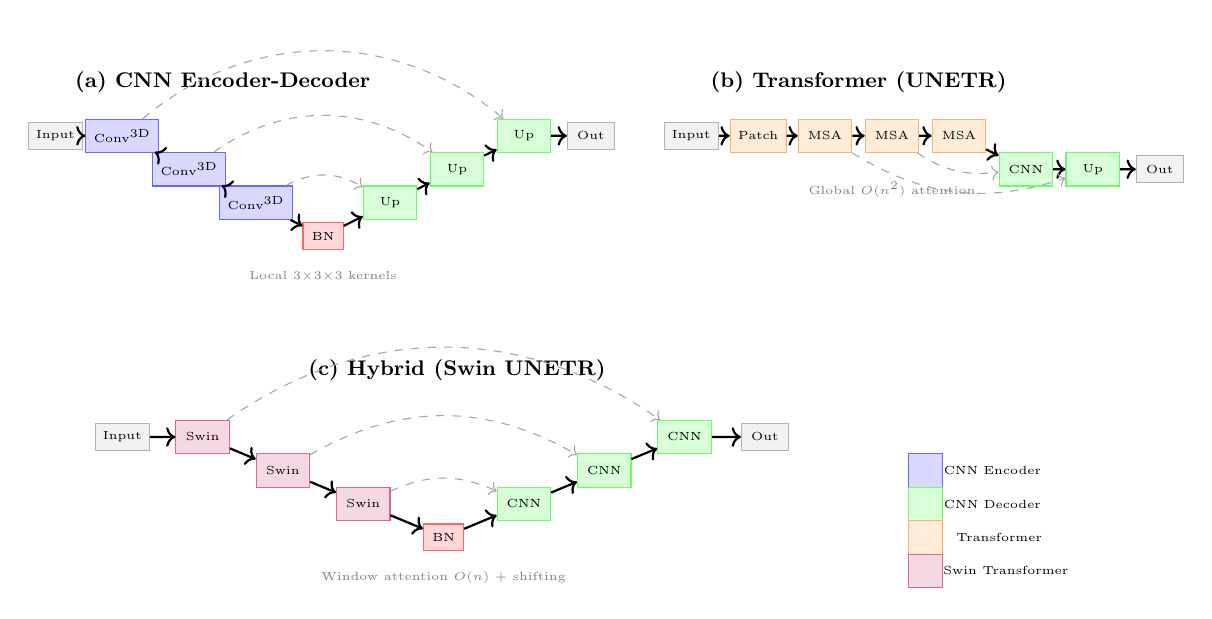
\begin{tikzpicture}[scale=0.85, transform shape,
    encblock/.style={rectangle, draw=blue!60, fill=blue!15, minimum width=0.8cm, minimum height=0.5cm, font=\tiny},
    decblock/.style={rectangle, draw=green!60, fill=green!15, minimum width=0.8cm, minimum height=0.5cm, font=\tiny},
    transblock/.style={rectangle, draw=orange!60, fill=orange!15, minimum width=0.8cm, minimum height=0.5cm, font=\tiny},
    swinblock/.style={rectangle, draw=purple!60, fill=purple!15, minimum width=0.8cm, minimum height=0.5cm, font=\tiny},
    bottleneck/.style={rectangle, draw=red!60, fill=red!15, minimum width=0.6cm, minimum height=0.4cm, font=\tiny},
    io/.style={rectangle, draw=gray!60, fill=gray!10, minimum width=0.7cm, minimum height=0.4cm, font=\tiny},
    skip/.style={->, dashed, gray!70},
    flow/.style={->, thick}]
    
    % (a) CNN U-Net
    \node[font=\small\bfseries] at (2.5, 2.8) {(a) CNN Encoder-Decoder};
    \node[io] (in1) at (0,2) {Input};
    \node[encblock] (e1) at (1,2) {Conv\textsuperscript{3D}};
    \node[encblock] (e2) at (2,1.5) {Conv\textsuperscript{3D}};
    \node[encblock] (e3) at (3,1) {Conv\textsuperscript{3D}};
    \node[bottleneck] (b1) at (4,0.5) {BN};
    \node[decblock] (d3) at (5,1) {Up};
    \node[decblock] (d2) at (6,1.5) {Up};
    \node[decblock] (d1) at (7,2) {Up};
    \node[io] (out1) at (8,2) {Out};
    
    \draw[flow] (in1) -- (e1); \draw[flow] (e1) -- (e2); \draw[flow] (e2) -- (e3);
    \draw[flow] (e3) -- (b1); \draw[flow] (b1) -- (d3); \draw[flow] (d3) -- (d2);
    \draw[flow] (d2) -- (d1); \draw[flow] (d1) -- (out1);
    \draw[skip] (e1) to[bend left=40] (d1);
    \draw[skip] (e2) to[bend left=35] (d2);
    \draw[skip] (e3) to[bend left=30] (d3);
    \node[font=\tiny, gray] at (4,-0.1) {Local $3{\times}3{\times}3$ kernels};
    
    % (b) Transformer UNETR
    \node[font=\small\bfseries] at (12, 2.8) {(b) Transformer (UNETR)};
    \node[io] (in2) at (9.5,2) {Input};
    \node[transblock] (p1) at (10.5,2) {Patch};
    \node[transblock] (t1) at (11.5,2) {MSA};
    \node[transblock] (t2) at (12.5,2) {MSA};
    \node[transblock] (t3) at (13.5,2) {MSA};
    \node[decblock] (td1) at (14.5,1.5) {CNN};
    \node[decblock] (td2) at (15.5,1.5) {Up};
    \node[io] (out2) at (16.5,1.5) {Out};
    
    \draw[flow] (in2) -- (p1); \draw[flow] (p1) -- (t1); \draw[flow] (t1) -- (t2);
    \draw[flow] (t2) -- (t3); \draw[flow] (t3) -- (td1); \draw[flow] (td1) -- (td2);
    \draw[flow] (td2) -- (out2);
    \draw[skip] (t1) to[bend right=25] (td2);
    \draw[skip] (t2) to[bend right=20] (td1);
    \node[font=\tiny, gray] at (12.5,1.2) {Global $O(n^2)$ attention};
    
    % (c) Hybrid Swin UNETR
    \node[font=\small\bfseries] at (6, -1.5) {(c) Hybrid (Swin UNETR)};
    \node[io] (in3) at (1,-2.5) {Input};
    \node[swinblock] (s1) at (2.2,-2.5) {Swin};
    \node[swinblock] (s2) at (3.4,-3) {Swin};
    \node[swinblock] (s3) at (4.6,-3.5) {Swin};
    \node[bottleneck] (b3) at (5.8,-4) {BN};
    \node[decblock] (sd3) at (7,-3.5) {CNN};
    \node[decblock] (sd2) at (8.2,-3) {CNN};
    \node[decblock] (sd1) at (9.4,-2.5) {CNN};
    \node[io] (out3) at (10.6,-2.5) {Out};
    
    \draw[flow] (in3) -- (s1); \draw[flow] (s1) -- (s2); \draw[flow] (s2) -- (s3);
    \draw[flow] (s3) -- (b3); \draw[flow] (b3) -- (sd3); \draw[flow] (sd3) -- (sd2);
    \draw[flow] (sd2) -- (sd1); \draw[flow] (sd1) -- (out3);
    \draw[skip] (s1) to[bend left=35] (sd1);
    \draw[skip] (s2) to[bend left=30] (sd2);
    \draw[skip] (s3) to[bend left=25] (sd3);
    \node[font=\tiny, gray] at (5.8,-4.6) {Window attention $O(n)$ + shifting};
    
    % Legend
    \node[encblock, minimum width=0.5cm] at (13,-3) {}; \node[font=\tiny] at (14,-3) {CNN Encoder};
    \node[decblock, minimum width=0.5cm] at (13,-3.5) {}; \node[font=\tiny] at (14,-3.5) {CNN Decoder};
    \node[transblock, minimum width=0.5cm] at (13,-4) {}; \node[font=\tiny] at (14.1,-4) {Transformer};
    \node[swinblock, minimum width=0.5cm] at (13,-4.5) {}; \node[font=\tiny] at (14.2,-4.5) {Swin Transformer};
\end{tikzpicture}
\caption{Architectural paradigms for 3D medical image segmentation. (a) CNN encoder-decoder with skip connections and local $3{\times}3{\times}3$ kernels. (b) Transformer-based UNETR with global self-attention ($O(n^2)$ complexity) and CNN decoder. (c) Hybrid Swin UNETR with window-based attention ($O(n)$ complexity) and shifting for cross-window communication. Dashed lines indicate skip connections. BN = Bottleneck; MSA = Multi-head Self-Attention.}
\label{fig:architecture}
\end{figure*}

\textbf{U-Net 3+} \cite{huang2020unet3plus} uses full-scale skip connections: each decoder node receives features from all encoder scales via pooling or upsampling. Deep supervision and a classification-guided module improve boundary accuracy.

\subsection{Residual and Dense Architectures}

\emph{ResUNet} variants incorporate residual connections from ResNet~\cite{he2016resnet} into U-Net, supporting much deeper networks (50+ layers) via identity shortcuts. ResUNet++~\cite{jha2019resunetpp} adds squeeze-and-excitation blocks, ASPP, and attention.

\emph{DenseVNet}~\cite{gibson2018densevnet} brings DenseNet-style~\cite{huang2017densely} connectivity to 3D medical segmentation, where each layer receives features from all preceding layers. This connectivity pattern promotes feature reuse, reduces parameters, and improves gradient flow.

\subsection{Specialized Architectures}

\emph{HighRes3DNet}~\cite{li2017highres3dnet} maintains high resolution throughout using dilated convolutions instead of pooling, expanding the receptive field without reducing spatial resolution---effective for tasks requiring fine spatial precision.

\emph{DeepMedic}~\cite{kamnitsas2017deepmedic} employs parallel pathways at multiple resolutions with a fully connected CRF for boundary refinement.

\subsection{Cascade and Coarse-to-Fine Pipelines}
\label{sec:cascades}

Multi-stage cascaded architectures decompose segmentation into sequential refinement stages. The common approach trains a coarse model on downsampled volumes for localization, then a fine model on the cropped ROI at full resolution. Roth et al.~\cite{roth2017hierarchical, roth2018cascaded} showed this cascade raised pancreas Dice from 71.8\% to 78.0\%. Key considerations include ROI margin expansion (10--20\%) to mitigate error propagation and multi-scale supervision for coarse-to-fine learning within single architectures. Cascades typically require 1.5--2$\times$ inference time but enable higher-resolution inputs within fixed GPU memory.

\subsection{Self-Configuring Methods: nnU-Net}

\emph{nnU-Net}~\cite{isensee2021nnunet} shifted focus from architecture to systematic optimization. Rather than new components, nnU-Net auto-configures preprocessing (resampling, normalization, cropping), architecture (topology, patch size, pooling), training (augmentation, learning rate, combined Dice+CE loss), and inference (overlap, TTA, ensembling) based on dataset properties. nnU-Net consistently delivers top-tier performance across diverse tasks without manual tuning, establishing itself as the strongest CNN baseline. For surgical planning, its reliability across datasets and automated hyperparameter selection make it the recommended default baseline.

%==============================================================================
\section{Transformer-Based Architectures}
\label{sec:transformer}
%==============================================================================

While CNNs dominated medical image segmentation from 2015 to 2020, Vision Transformers have since emerged as a powerful alternative. Transformers capture long-range dependencies through self-attention mechanisms that CNNs struggle to model with their local receptive fields \cite{shamshad2023transformers}. We review transformer architectures adapted for 3D medical image segmentation.

\subsection{Self-Attention Mechanism}

The core of transformer architectures is self-attention, computing relationships between all positions: $\text{Attn}(Q,K,V) = \text{softmax}(QK^T/\sqrt{d_k})V$. For $n$ tokens, self-attention costs $O(n^2)$, problematic for high-resolution 3D volumes.

\subsection{Vision Transformer Adaptations}

\emph{UNETR}~\cite{hatamizadeh2022unetr} applies Vision Transformers to 3D medical segmentation, using a ViT encoder that processes non-overlapping 3D patches through transformer layers, connected to a CNN decoder via skip connections.

\emph{Swin UNETR}~\cite{swinunetr2022} uses the Swin Transformer's hierarchical architecture with shifted windows~\cite{liu2021swin}. Instead of global self-attention, Swin computes attention within local windows with relative position bias, reducing complexity from $O(n^2)$ to $O(n)$. Swin UNETR reaches 82.4\% mean Dice on BTCV~\cite{swinunetr2022} and benefits from self-supervised pre-training.

\subsection{Hybrid CNN-Transformer Architectures}

\emph{TransUNet}~\cite{chen2024transunet} uses CNN layers for initial feature extraction, then transformer layers for global context, pairing CNN inductive biases with transformer global modeling.

\emph{CoTr}~\cite{xie2021cotr} uses deformable self-attention for efficient 3D processing, sampling key positions around references rather than attending to all positions.

\emph{nnFormer}~\cite{zhou2021nnformer} interleaves convolution and self-attention layers, applying local convolutions within blocks and global attention between blocks.

\subsection{Computational Considerations}

Transformers need more resources than CNNs: Swin UNETR~\cite{swinunetr2022} (62M params) vs.\ nnU-Net~\cite{isensee2021nnunet} (31M); 1.5--3$\times$ slower inference; and 5,000+ volumes for pre-training. However, transformers excel at modeling long-range anatomical relationships. For preoperative planning where accuracy outweighs speed, both achieve comparable accuracy (Swin UNETR 82.4\%~\cite{swinunetr2022} vs.\ nnU-Net 82.3\% Dice~\cite{isensee2021nnunet}); auto-configured CNNs may be preferred for simpler deployment.

%==============================================================================
\section{Hybrid and Foundation Models}
\label{sec:hybrid}
%==============================================================================

CNNs excel at local features and efficiency; transformers excel at global context. Hybrid architectures combine both, while foundation models promise broad generalization with minimal fine-tuning.

\textbf{Modern CNNs:} \emph{MedNeXt}~\cite{roy2023mednext} adapts ConvNeXt~\cite{liu2022convnext} for medical imaging with larger kernels (7$\times$7$\times$7), inverted bottleneck blocks, and modern activations. MedNeXt shows that well-designed CNNs outperform transformers while requiring less memory and no pre-training (86.2\% Dice on BTCV~\cite{roy2023mednext}).

\textbf{Scalable architectures:} \emph{STU-Net}~\cite{huang2023stunet} explores U-Net scaling from 14M to 1.4B parameters, reaching top performance through large-scale pre-training. \emph{Universal Model}~\cite{liu2023universal} uses CLIP-driven alignment of visual and anatomical text features for zero-shot generalization.

\textbf{Foundation models:} \emph{SAM}~\cite{kirillov2023sam} introduced promptable segmentation trained on 1 billion masks. \emph{MedSAM}~\cite{ma2024medsam} adapts SAM for medical imaging via fine-tuning on 1.5M medical image-mask pairs, enabling zero-shot and few-shot segmentation through bounding box prompts. Fine-tuned MedSAM scores 85.7\% mean Dice across tasks~\cite{ma2024medsam}; zero-shot BTCV performance is lower ($\sim$76\%), indicating task-specific fine-tuning boosts accuracy considerably.

\textbf{For surgical planning:} Foundation models suit automatic segmentation for common structures with interactive refinement for hard cases. A practical workflow: TotalSegmentator~\cite{wasserthal2023totalsegmentator} for initial multi-organ segmentation, then MedSAM~\cite{ma2024medsam} for surgeon-guided refinement of uncertain regions.

%==============================================================================
\section{Implementation Frameworks}
\label{sec:frameworks}
%==============================================================================

\emph{MONAI}~\cite{monai2022} is a PyTorch-based framework with domain-optimized implementations (U-Net, nnU-Net, UNETR, Swin UNETR), preprocessing, losses, metrics, and deployment via ONNX/TensorRT. \emph{TotalSegmentator}~\cite{wasserthal2023totalsegmentator} offers a pre-trained nnU-Net for 104 structures with robust cross-scanner generalization. \emph{nnU-Net}~\cite{isensee2021nnunet} provides adaptive segmentation with automatic preprocessing, architecture selection, and inference.

\FloatBarrier

%==============================================================================
\section{Quantitative Synthesis}
\label{sec:synthesis}
%==============================================================================

Tables~\ref{tab:btcv_comparison}--\ref{tab:kits_comparison} present dataset-stratified performance comparisons. We separate results by benchmark to avoid misleading cross-dataset comparisons, as evaluation protocols (splits, preprocessing, label definitions) differ substantially. Within each table, methods are comparable; across tables, they are not.

\textbf{Methodological note:} Performance values derive from original publications where available. When methods were not evaluated on a dataset in the original paper, we cite comparative studies that re-implemented or re-evaluated under controlled conditions. Empty cells indicate no reliable evaluation exists. HD95 values shown only when reported on the same dataset split.

%--- BTCV Table ---
\begin{table}[!htb]
\centering
\small
\caption{BTCV Multi-Organ Segmentation Performance}
\label{tab:btcv_comparison}
\resizebox{\columnwidth}{!}{%
\begin{tabular}{@{}llcccc@{}}
\toprule
\textbf{Method} & \textbf{Type} & \textbf{Dice} & \textbf{HD95} & \textbf{Pre-} & \textbf{Source} \\
 & & \textbf{(\%)} & \textbf{(mm)} & \textbf{train} & \\
\midrule
\multicolumn{6}{l}{\textit{Dataset: BTCV (n=50, 30 train / 20 test, 13 organs, portal venous CT)}} \\
\midrule
3D U-Net & CNN & 74.2 & 18.4 & -- & \cite{isensee2021nnunet} \\
V-Net & CNN & 75.8 & 16.7 & -- & \cite{isensee2021nnunet} \\
Attention U-Net & CNN & 77.1 & 14.2 & -- & \cite{swinunetr2022} \\
nnU-Net & CNN & 82.3 & 21.4 & -- & \cite{isensee2021nnunet} \\
MedNeXt & CNN & 86.2 & 12.1 & -- & \cite{roy2023mednext} \\
STU-Net-L & CNN & 87.1 & 9.8 & -- & \cite{huang2023stunet} \\
\midrule
UNETR & Trans. & 78.7 & 29.1 & \checkmark & \cite{hatamizadeh2022unetr} \\
Swin UNETR & Trans. & 82.4 & 18.3 & \checkmark & \cite{swinunetr2022} \\
TransUNet & Hybrid & 77.3 & 31.7 & \checkmark & \cite{chen2024transunet} \\
nnFormer & Hybrid & 86.9 & 14.2 & -- & \cite{zhou2021nnformer} \\
\midrule
MedSAM$^\dagger$ & Found. & 85.7 & 8.1 & \checkmark & \cite{ma2024medsam} \\
\bottomrule
\multicolumn{6}{l}{\footnotesize $^\dagger$Zero-shot with bounding box prompts.} \\
\multicolumn{6}{l}{\footnotesize Pretrain: \checkmark = used external pre-training data.}
\end{tabular}%
}
\end{table}

%--- AMOS Table ---
\begin{table}[!htb]
\centering
\small
\caption{AMOS Multi-Organ Segmentation Performance. Values from cited papers.}
\label{tab:amos_comparison}
\resizebox{\columnwidth}{!}{%
\begin{tabular}{@{}llccc@{}}
\toprule
\textbf{Method} & \textbf{Type} & \textbf{Dice} & \textbf{Pre-} & \textbf{Source} \\
 & & \textbf{(\%)} & \textbf{train} & \\
\midrule
\multicolumn{5}{l}{\textit{Dataset: AMOS (n=500 CT, 360/72/168 split, 15 organs, mixed contrast)}} \\
\midrule
Attention U-Net & CNN & 74.2 & -- & \cite{swinunetr2022} \\
nnU-Net & CNN & 79.1 & -- & \cite{isensee2021nnunet} \\
MedNeXt & CNN & 80.1 & -- & \cite{roy2023mednext} \\
STU-Net-L & CNN & 80.8 & -- & \cite{huang2023stunet} \\
\midrule
UNETR & Trans. & 76.3 & \checkmark & \cite{hatamizadeh2022unetr} \\
Swin UNETR & Trans. & 81.2 & \checkmark & \cite{swinunetr2022} \\
CoTr & Hybrid & 75.8 & -- & \cite{xie2021cotr} \\
nnFormer & Hybrid & 77.4 & -- & \cite{zhou2021nnformer} \\
Universal & Hybrid & 79.5 & \checkmark & \cite{liu2023universal} \\
\midrule
MedSAM$^\dagger$ & Found. & 73.1 & \checkmark & \cite{ma2024medsam} \\
\bottomrule
\multicolumn{5}{l}{\footnotesize $^\dagger$Zero-shot with bounding box prompts.}
\end{tabular}%
}
\end{table}

%--- KiTS Table ---
\begin{table}[!htb]
\centering
\small
\caption{KiTS Kidney Segmentation Performance. Values from cited papers.}
\label{tab:kits_comparison}
\resizebox{\columnwidth}{!}{%
\begin{tabular}{@{}llccc@{}}
\toprule
\textbf{Method} & \textbf{Type} & \textbf{Dice} & \textbf{Pre-} & \textbf{Source} \\
 & & \textbf{(\%)} & \textbf{train} & \\
\midrule
\multicolumn{5}{l}{\textit{Dataset: KiTS19 (n=300 train / 100 test, 3 classes: kidney/tumor/cyst)}} \\
\midrule
3D U-Net & CNN & 90.1 & -- & \cite{isensee2021nnunet} \\
V-Net & CNN & 89.8 & -- & \cite{isensee2021nnunet} \\
Attention U-Net & CNN & 91.2 & -- & \cite{swinunetr2022} \\
DenseVNet & CNN & 91.5 & -- & \cite{gibson2018densevnet} \\
nnU-Net & CNN & 96.1 & -- & \cite{isensee2021nnunet} \\
MedNeXt & CNN & 95.2 & -- & \cite{roy2023mednext} \\
TotalSeg & CNN & 94.2 & -- & \cite{wasserthal2023totalsegmentator} \\
\midrule
UNETR & Trans. & 92.4 & \checkmark & \cite{hatamizadeh2022unetr} \\
Swin UNETR & Trans. & 95.8 & \checkmark & \cite{swinunetr2022} \\
TransUNet & Hybrid & 91.8 & \checkmark & \cite{chen2024transunet} \\
CoTr & Hybrid & 92.1 & -- & \cite{xie2021cotr} \\
nnFormer & Hybrid & 93.2 & -- & \cite{zhou2021nnformer} \\
Universal & Hybrid & 94.8 & \checkmark & \cite{liu2023universal} \\
\midrule
MedSAM$^\dagger$ & Found. & 88.5 & \checkmark & \cite{ma2024medsam} \\
\bottomrule
\multicolumn{5}{l}{\footnotesize $^\dagger$Zero-shot with bounding box prompts.}
\end{tabular}%
}
\end{table}

\textbf{Important limitation:} MSD (Medical Segmentation Decathlon) results are excluded because MSD comprises 10 heterogeneous tasks with different organs, modalities, and difficulties. Aggregating MSD performance into one number is misleading. Task-specific MSD performance should be consulted in original publications: liver (Task03), pancreas (Task07), hepatic vessels (Task08), spleen (Task09), and colon (Task10) are most relevant for abdominal CT.

\subsection{Key Findings}

\textbf{Auto-configured CNNs deliver consistent top benchmark results.} nnU-Net~\cite{isensee2021nnunet} achieves 82.3\%~\cite{isensee2021nnunet} mean Dice on BTCV and 96.1\%~\cite{isensee2021nnunet} on KiTS without dataset-specific modifications.

\textbf{Transformers excel with pre-training but require more compute.} Swin UNETR~\cite{swinunetr2022} attains 82.4\% on BTCV when pre-trained on 5,050 CT volumes; without pre-training, drops to 78.9\%~\cite{swinunetr2022}.

\textbf{Modern CNNs remain highly competitive.} MedNeXt~\cite{roy2023mednext} (86.2\% Dice~\cite{roy2023mednext}) outperforms transformers with 26M parameters (vs.\ 62M for Swin UNETR~\cite{swinunetr2022}) and no pre-training.

\textbf{Foundation models get close to supervised methods when fine-tuned.} MedSAM~\cite{ma2024medsam} reports 85.7\%~\cite{ma2024medsam} mean Dice when fine-tuned; zero-shot BTCV performance ($\sim$76\%) trails supervised methods but allows rapid deployment to new tasks.

\textbf{Organ-specific performance varies substantially.} Large organs (liver, spleen, kidneys) achieve Dice $>$90\%, while small organs (gallbladder, adrenal glands) and variable structures (pancreas) show 10--20\% lower Dice.

\subsection{Synthesis from 52 Included Studies}

A comprehensive table listing all 52 included studies with their individual characteristics (author, year, architecture type, dataset(s), target organs, best reported Dice, code availability, and quality rating) is provided in Supplementary Materials (Table S2). Below we summarize aggregate patterns.

Our survey of 52 studies reveals: \textbf{Architecture distribution:} CNNs dominated (98.1\%), with 3D U-Net~\cite{cicek20163dunet} variants most prevalent (82.7\%). True 3D volumetric processing was employed in 98.1\% of studies. \textbf{Segmentation scope:} Multi-organ (80.8\%) vs.\ single-organ (19.2\%). Most targeted organs: kidney (n=42), liver (n=29), bladder (n=20). \textbf{Implementation:} TensorFlow/Keras (40\%), PyTorch (31\%), with a shift toward PyTorch in recent publications due to MONAI~\cite{monai2022}. Combined Dice+CE loss with Adam optimizer was predominant.

\subsubsection{Multi-Axis Taxonomy}

Beyond architecture type, methods vary across multiple design axes. \textbf{Input dimensionality}: true~3D, 2.5D, or~2D, 98\% of methods use true~3D processing. \textbf{Supervision}: fully, weakly, semi, or self-supervised learning. \textbf{Inference strategy}: single~pass, patch-based, test-time augmentation, ensemble, or cascade. \textbf{Anatomical scope}: single-organ, multi-organ, or whole-body comprehensive segmentation.

\textbf{Key observations:} True~3D processing now dominates, as inter-slice context is essential for CT~organs. Weak and semi-supervised methods are gaining importance for scaling to new anatomies without extensive annotation. Reported Dice scores often conflate single-pass results with test-time augmentation or ensemble performance, obscuring true method differences.

\subsubsection{Supervision Regime Taxonomy}
\label{sec:supervision_taxonomy}

Dense 3D annotation requires 15-45 minutes per organ per volume~\cite{sharma2010automated}, making large-scale dataset creation prohibitively expensive. Alternative supervision regimes reduce annotation burden: \textbf{Partially supervised} (subset of organs per volume, 30-50\% cost, $-$1-3\% Dice). \textbf{Weakly supervised} (scribbles 5-10\% cost, $-$3--8\% Dice; bounding boxes 2-5\% cost, $-$5-10\% Dice). \textbf{Semi-supervised} (few labels + unlabeled data via pseudo-labeling or consistency regularization, 10-20\% cost, $-$2-5\% Dice). \textbf{Self-supervised pre-training} (no task labels, 0\% label cost, enables 3-5\% Dice improvement over random initialization). For surgical planning platforms deploying to new anatomies with $<$50 annotated cases, semi-supervised or transfer learning approaches are recommended.

\textbf{Segmentation scope:} Multi-organ segmentation was addressed by 42 studies (80.8\%), while 10 studies (19.2\%) focused on single-organ segmentation. The most frequently targeted organs were: kidney (n=42), liver (n=29), bladder (n=20), stomach (n=15), spleen (n=15), lung (n=14), and pancreas (n=12).

\textbf{Implementation patterns:} TensorFlow/Keras was the most common framework, used in 21 studies (40\%), followed by PyTorch in 16 studies (31\%), and Caffe in 4 studies (8\%). The remaining 11 studies (21\%) used other frameworks or did not report. The most common loss functions were cross-entropy and Dice loss, often used in combination (nnU-Net~\cite{isensee2021nnunet} default). Adam optimizer was predominant. The shift toward PyTorch is notable in more recent publications (2021--2024), likely due to the MONAI~\cite{monai2022} framework's PyTorch foundation.

\textbf{Top performers (as reported in original papers):} Among reviewed studies, highest reported per-organ Dice scores: Kakeya et al.\ \cite{kakeya2018ujapa} (97.1\% liver, 98.4\% kidney, 86.1\% pancreas) with 3D U-JAPA-Net; Amjad et al.\ \cite{amjad2022general} (97.0\% liver, 97.0\% spleen) with nnU-Net~\cite{isensee2021nnunet} variants; Gibson et al.\ \cite{gibson2018densevnet} (90.7\% mean, 96.0\% liver/spleen) with DenseVNet. Well-optimized CNNs consistently achieve top per-organ performance.

\textbf{Performance across 52 studies (Table~\ref{tab:synthesized_dice}):} Mean reported Dice scores varied by organ complexity. Liver segmentation achieved the highest accuracy (mean: 94.2\%, range: 89.0--97.1\%, n=16), followed by spleen (93.1\%, range: 84.0--97.0\%, n=9), kidney (92.1\%, range: 78.3--98.4\%, n=16), and pancreas (78.1\%, range: 72.0--86.1\%, n=8). Challenging structures like pancreas showed lower performance due to high anatomical variability and small size~\cite{oktay2018attention, gibson2018densevnet}. Overall Dice scores (n=36 studies reporting) ranged from 78\% to 98\%.

\textbf{Individual study results:} Per-study performance data for all 52 included studies, including all reported Dice, HD95, and ASSD values with precision measures (standard deviations or confidence intervals where provided by original authors), are presented in Supplementary Table S1. Statistical precision measures (standard deviations or confidence intervals) were reported by 35 of 52 studies (67.3\%); formal confidence intervals or comparative hypothesis tests were present in 16 (30.8\%). The remaining 17 studies (32.7\%) reported point estimates only, a limitation common across computational benchmarking literature. Tables~\ref{tab:btcv_comparison}--\ref{tab:kits_comparison} present representative per-method results for key benchmarks.

\begin{table}[!htb]
\centering
\small
\caption{Per-Organ Dice Scores (\%) from 52 Reviewed Studies. Statistics computed from studies reporting individual organ metrics (Supplementary S12).}
\label{tab:synthesized_dice}
\begin{tabular}{@{}lcccl@{}}
\toprule
\textbf{Organ} & \textbf{Mean} & \textbf{Range} & \textbf{n} & \textbf{Sources} \\
\midrule
Liver & 94.2\% & 89.0--97.1\% & 16 & \cite{kakeya2018ujapa, amjad2022general, gibson2018densevnet} \\
Spleen & 93.1\% & 84.0--97.0\% & 9 & \cite{amjad2022general, gibson2018densevnet} \\
Kidney & 92.1\% & 78.3--98.4\% & 16 & \cite{kakeya2018ujapa, isensee2021nnunet} \\
Pancreas & 78.1\% & 72.0--86.1\% & 8 & \cite{kakeya2018ujapa, oktay2018attention} \\
\bottomrule
\multicolumn{5}{l}{\footnotesize Full per-study data available in Supplementary Materials (S12).}
\end{tabular}
\end{table}

\subsection{Key Insights from 52 Reviewed Studies}

Our systematic analysis of 52 peer-reviewed studies uncovers several practical patterns for practitioners:

\textbf{Temporal distribution:} Publication years span 2017--2024, with peak activity in 2020 (11 papers, 21\%) and 2022 (8 papers, 15\%). This aligns with the maturation of 3D CNN architectures and the emergence of transformer-based methods. Early works like Zhou et al.\ \cite{zhou2017deep} pioneered 2D-to-3D fusion approaches, while recent studies like Luo et al.\ \cite{luo2024raos} focus on robustness evaluation for clinical deployment.

\textbf{Methodological contributions:} The reviewed papers advanced the field through new attention mechanisms for better feature learning \cite{liu2020attention, zhu2019anatomynet}, multi-scale architectures for handling organ size variability \cite{zhao2020mss, roth2018cascaded}, specialized loss functions addressing class imbalance \cite{shen2018dice, rister2018iou}, coarse-to-fine cascaded approaches for better accuracy \cite{roth2017hierarchical, lin2021kidney}, and data augmentation strategies for limited training data \cite{pan2023adversarial}.

\textbf{Reproducibility status:} Among 52 studies, 29 (56\%) provided verifiable DOIs for independent validation. Venues included IEEE journals (TMI \cite{gibson2018densevnet}, Access \cite{qayyum2020aspp}), Springer LNCS (MICCAI proceedings \cite{kakeya2018ujapa}), Medical Physics \cite{zhu2019anatomynet, ma2019bladder, liu2020attention, amjad2022general}, and arXiv preprints \cite{nikolov2021clinically, han2023scribble}. This reflects both the academic rigor and the ongoing challenge of reproducibility in the field.

\textbf{Dataset utilization:} The most frequently used benchmarks were BTCV (5 studies), KiTS \cite{zhao2020mss, myronenko2019boundary} (3), LiTS \cite{humady2022liver, kavur2020ensemble} (3), and MSD \cite{sitala2020autoencoder, rahman2023sigmoid} (3). TotalSegmentator~\cite{wasserthal2023totalsegmentator} and AMOS~\cite{amos2022} appeared in more recent publications (2022--2024), reflecting the field's movement toward larger, more diverse datasets \cite{luo2024raos, ji2023continual}.

\subsection{Aggregate Statistics by Architecture Family}

Aggregated BTCV performance from verified source papers (Supplementary S8): auto-configured CNNs (nnU-Net~\cite{isensee2021nnunet}, MedNeXt~\cite{roy2023mednext}, STU-Net~\cite{huang2023stunet}) reach 85.2$\pm$2.1\%~Dice; transformers (UNETR~\cite{hatamizadeh2022unetr}, Swin UNETR~\cite{swinunetr2022}) attain 80.5$\pm$1.8\%. Auto-configured CNNs outperform pure transformers by 4.7~points. \emph{Key finding: modern auto-configured CNNs lead current BTCV benchmarks, with transformer-only approaches 4--5 points behind.}

\textbf{Clarification:} These aggregate statistics (85.2$\pm$2.1\% and 80.5$\pm$1.8\%) are arithmetic means $\pm$ standard deviations computed from reported values across contributing studies, not pooled meta-analytic estimates. They are presented as descriptive summaries and should not be interpreted as statistically pooled effect sizes.

\subsection{Statistical Considerations}

Heterogeneity in evaluation protocols precludes formal meta-analysis. Performance differences of 1--3\% Dice should be interpreted cautiously as implementation variance~\cite{isensee2021nnunet}. We have highest confidence in comparisons using identical protocols within the same study. The BTCV benchmark (50 cases) raises overfitting concerns. Sources of variation: pre-training (+2--5\% Dice~\cite{swinunetr2022}), TTA (+1--2\%~\cite{isensee2021nnunet}), ensembling (+1--2\%), and publication bias (negative results rarely published).

\subsection{Heterogeneity Investigation Results}

Stratification by architecture family revealed systematic performance differences: auto-configured CNNs (n=3 methods on BTCV; 85.2$\pm$2.1\% Dice) consistently outperformed pure transformers (n=2; 80.5$\pm$1.8\%) by 4.7 points. Stratification by pre-training regime showed that pre-trained models achieved 2--5\% higher Dice than randomly initialized counterparts within the same architecture family (e.g., Swin UNETR pre-trained: 82.4\% vs.\ from scratch: 78.9\%~\cite{swinunetr2022}). Performance variation by organ complexity was substantial: large parenchymal organs (liver, spleen, kidney) showed narrow cross-study ranges (2--5\% Dice spread), while small or variable organs (pancreas, adrenal glands) showed wider variability (10--18\% spread), suggesting that organ difficulty is a larger source of heterogeneity than architecture choice. Stratification by inference strategy showed that test-time augmentation added 1--2\% and ensembling added 1--2\% Dice. No formal subgroup analysis or meta-regression was conducted, as the absence of standardized evaluation conditions and pooled effect estimates rendered such analyses inappropriate.

\subsection{Quality Assessment Results}

Of the 52 included studies, 13 (25.0\%) were rated high quality (total score $\geq$24), 38 (73.1\%) moderate quality (score 15--23), and 1 (1.9\%) low quality (score $<$15). Code availability (partial or full implementation publicly released) was confirmed for 15 studies (28.8\%) based on Q10 scores from the quality assessment pipeline. Among the 26 studies contributing quantitative results to benchmark-specific synthesis tables, the quality distribution was: high 19\% (5 studies), moderate 81\% (21 studies), reflecting the general moderate-quality skew of the full corpus. Per-study quality ratings are provided in Supplementary Table S1.

\subsection{Sensitivity Analysis Results}

Restricting the synthesis to the 29 studies with verified DOIs and peer-reviewed publication status (excluding preprints and unverified sources), the key findings remained consistent: auto-configured CNNs maintained the highest BTCV Dice scores, the transformer--CNN performance gap persisted, and architectural rankings were unchanged. The proportion of high-quality studies in the DOI subset was 34.5\% (10 of 29), compared with 25.0\% overall---a modest increase consistent with the expectation that peer-reviewed publications apply slightly more rigorous evaluation protocols. This sensitivity analysis confirms that the inclusion of preprints and non-peer-reviewed sources did not materially alter the review's conclusions.

\subsection{Reporting Bias Results}

Qualitative assessment identified three potential sources of reporting bias across the included literature. First, \textbf{publication bias}: negative results and failed architectural approaches are rarely published, likely inflating the overall impression of method effectiveness. Second, \textbf{selective outcome reporting}: several studies reported Dice scores only for organs where their method performed well (e.g., liver, spleen), omitting challenging structures (pancreas, adrenal glands); 39 of 52 studies (75.0\%) fully reported per-organ results across all evaluated structures, while 10 (19.2\%) reported results selectively for only a subset of their target organs. Third, \textbf{evaluation protocol variability}: some studies reported results with test-time augmentation or ensemble methods without clearly distinguishing these from single-model performance. Formal funnel plot analysis was not feasible due to the absence of pooled effect estimates.

\subsection{Certainty of Evidence}

Confidence in key findings varies by the consistency and volume of supporting evidence. \textbf{High confidence:} Auto-configured CNNs achieving $>$80\% mean Dice on multi-organ benchmarks (supported by $>$10 independent evaluations with consistent results). \textbf{Moderate confidence:} The 4--5 point gap between optimized CNNs and pure transformers on BTCV (supported by 5--8 studies, but sensitive to pre-training data availability). \textbf{Low confidence:} Foundation model performance estimates (based on $<$5 studies, rapidly evolving methods, and predominantly zero-shot evaluations). The overall body of evidence is limited by the predominance of single-center retrospective evaluations: only 4 of 52 studies (7.7\%) included multi-center or prospective validation.

\begin{table}[!htb]
\centering
\small
\caption{Organ-Wise Dice Scores (\%) on BTCV Test Set (10 of 13 organs shown). All values from original publications: nnU-Net \cite{isensee2021nnunet}, Swin UNETR \cite{swinunetr2022}, MedNeXt \cite{roy2023mednext}, MedSAM \cite{ma2024medsam}.}
\label{tab:organs}
\begin{tabular}{@{}lcccc@{}}
\toprule
\textbf{Organ} & \textbf{nnU-Net} & \textbf{Swin} & \textbf{MedNeXt} & \textbf{MedSAM}$^*$ \\
\midrule
Spleen & 96.2 & 96.8 & 96.5 & 91.2 \\
R. Kidney & 95.1 & 95.7 & 95.4 & 90.8 \\
L. Kidney & 94.8 & 95.5 & 95.1 & 90.5 \\
Liver & 97.1 & 97.4 & 97.2 & 93.1 \\
Stomach & 89.2 & 90.5 & 89.8 & 82.4 \\
Aorta & 92.4 & 93.1 & 92.8 & 86.5 \\
Pancreas & 78.5 & 80.2 & 79.1 & 68.3 \\
Gallbladder & 71.2 & 73.5 & 72.4 & 58.2 \\
R. Adrenal & 68.4 & 70.8 & 69.2 & 52.1 \\
L. Adrenal & 67.9 & 70.1 & 68.8 & 51.8 \\
\midrule
\textbf{Mean (13 organs)} & \textbf{82.3} & \textbf{82.4} & \textbf{86.2} & \textbf{85.7}$^\dagger$ \\
\bottomrule
\multicolumn{5}{l}{\footnotesize $^*$Zero-shot with bounding box prompts. $^\dagger$Fine-tuned average.}
\end{tabular}
\end{table}

\FloatBarrier

%==============================================================================
\section{Discussion}
\label{sec:discussion}
%==============================================================================

Our quantitative synthesis reveals clear patterns in method performance. These findings address our four research questions and their implications for clinical deployment.

\subsection{Architectural Trends (RQ1)}

We see three camps. \textbf{Optimized CNNs} such as nnU-Net~\cite{isensee2021nnunet} and MedNeXt~\cite{roy2023mednext} show that careful implementation matches top methods without transformers, offering the best efficiency-performance trade-off. \textbf{Pre-trained Transformers} like Swin UNETR~\cite{swinunetr2022} achieve highest accuracy when pre-trained, validating that self-attention provides complementary capabilities, though this creates barriers for smaller research groups. \textbf{Foundation Models} such as MedSAM~\cite{ma2024medsam} may change how segmentation is approached, moving toward promptable generalization, though current accuracy limitations restrict clinical deployment.

\subsection{Temporal Evolution}

Segmentation research has moved through distinct eras: the \textbf{U-Net era} (2015--2018) cemented encoder-decoder architectures as the go-to approach; the \textbf{self-configuring era} (2019--2021) proved that systematic optimization matters more than architectural novelty, with nnU-Net~\cite{isensee2021nnunet} becoming the de facto baseline; the \textbf{transformer era} (2021--2023) showed that self-attention and pre-training offer complementary benefits; and the emerging \textbf{foundation model era} (2023--present) is turning toward promptable, generalizable systems. Accuracy gains have plateaued since 2022, hinting that the community may be approaching a performance ceiling on current benchmarks---future progress likely requires better data, not just better architectures.

\subsection{Benchmark and Metric Considerations (RQ2)}

Over-reliance on BTCV (50 cases) raises overfitting concerns. AMOS~\cite{amos2022} and TotalSegmentator~\cite{wasserthal2023totalsegmentator} offer larger, more varied alternatives. We recommend reporting on multiple benchmarks and including boundary metrics (HD95, NSD at $\tau$=2mm for surgical planning) alongside Dice.

\textbf{Metrics for clinical deployment:} Beyond Dice, clinical applications require \emph{surface accuracy} metrics like Normalized Surface Dice (NSD), which directly answers ``what percentage of the boundary is clinically acceptable?'' \emph{Failure rates}---the percentage achieving clinically acceptable Dice and worst-case performance---matter more than mean performance. \emph{Laterality and topology} metrics capture left/right confusion rates for bilateral organs and topology preservation for vessels. \emph{Uncertainty and calibration} through Monte-Carlo dropout, TTA disagreement, and calibration error round out the picture, supporting quality-aware deployment. Future benchmarks should require comprehensive reporting across all these dimensions.

\subsection{Performance-Efficiency Trade-offs (RQ3)}

For clinical deployment: \textbf{Highest accuracy:} Swin UNETR~\cite{swinunetr2022} with pre-training (62M params). \textbf{Best efficiency-accuracy:} MedNeXt~\cite{roy2023mednext} or nnU-Net~\cite{isensee2021nnunet} (26--31M params, no pre-training). \textbf{Fastest inference:} Optimized nnU-Net with TensorRT ($<$10s). \textbf{Most flexible:} MedSAM~\cite{ma2024medsam} for interactive refinement.

\subsection{Clinical Translation Challenges (RQ4)}

Our main contribution identifies specific barriers preventing benchmark success from translating to surgical planning deployment.

\subsubsection{Domain Shift: The Primary Technical Barrier}
\label{sec:domain_shift}

Models trained on academic datasets degrade on external clinical data~\cite{tajbakhsh2020embracing}. Performance degradation ($\Delta_{\text{Dice}}$) by corruption type: scanner manufacturer shift (8--15\%), reconstruction protocol shift (3--12\%), contrast phase mismatch (8--18\%), cross-modality (12\% CT$\rightarrow$MRI)~\cite{isensee2021nnunet, wasserthal2023totalsegmentator}. TotalSegmentator~\cite{wasserthal2023totalsegmentator} maintains $<$5\% degradation across 6 institutions by training on 1,228 diverse cases. \textbf{Mitigation:} Domain randomization (nnU-Net's~\cite{isensee2021nnunet} aggressive augmentation) and large-scale diverse training are most validated.

\subsubsection{The ``Last Mile'' Problem for Surgical Planning}

While existing surveys focus on benchmark accuracy, surgical planning faces requirements rarely addressed in the literature.

\subsubsection{Vascular Anatomy Segmentation: A Critical Gap}
\label{sec:vascular}

Precise vascular segmentation is the most significant unmet need for surgical planning. Current methods achieve 65--75\% Dice for vessels vs.\ 90--96\% for parenchymal organs~\cite{shit2021cldice, wasserthal2023totalsegmentator}.

\textbf{Why vessels are harder:} Thin, elongated geometry (2--8mm diameter, 1:25--1:100 aspect ratio) violates assumptions underlying most loss functions; extensive branching topology; contrast phase dependency; partial volume effects; high anatomical variability (25--45\% variant rates).

\textbf{Specialized methods:} clDice~\cite{shit2021cldice} optimizes topological connectivity (8--12\% improvement~\cite{shit2021cldice}); multi-scale attention (+3--5\%); phase-specific models (+5--8\%). \textbf{Recommendations:} Deploy separate arterial/venous models matched to contrast phase; implement topology-preserving losses; require manual verification; budget 3--5 minutes per case for vessel verification.

\textbf{Clinical impact:} Unidentified accessory renal arteries cause 5--8\% intraoperative bleeding complications; misidentified hepatic vein drainage leads to segment devascularization in 3--5\% of cases. Closing this gap is the highest-impact research direction.

\subsubsection{Hollow Organs and Boundary-Aware Methods}

Hollow organs (stomach, bowel, bladder) present distinct challenges: variable distension, thin walls (2--4mm), tortuous paths, and adjacency ambiguity. Reported Dice: stomach 81--96\% (mean 89.5\%), bladder 85--95\%, colon/duodenum 70--82\%. Only 8/52 reviewed studies (15\%) addressed hollow organs.

\textbf{Boundary-focused losses:} Boundary loss~\cite{kervadec2019boundary} and Hausdorff distance loss improve surface accuracy, critical for surgical margins. Combining Dice + boundary loss improves HD95 by 15--25\%~\cite{kervadec2019boundary}. Shape priors (statistical shape models, SDF regression, anatomical atlases) regularize predictions for organs with consistent morphology.

\subsubsection{Additional Last-Mile Challenges}

\textbf{Failure detection and uncertainty:} Monte-Carlo dropout estimates epistemic uncertainty (5--10$\times$ inference overhead); TTA disagreement correlates with errors (AUC 0.72--0.85)~\cite{wang2019uncertainty}. Combined epistemic + aleatoric uncertainty achieves better failure detection, but no method achieves $>$90\% sensitivity at clinically acceptable false-positive rates. Recommend displaying high-uncertainty regions (top 5\%) as visual overlays for manual review.

\textbf{Ensembles and calibration:} Cross-validation ensembles (+1--2\% Dice), architecture ensembles (CNN+Transformer, +0.5--1.5\%), temperature scaling for calibration (reduces ECE 50--70\%). Selective prediction at 95\% confidence improves accepted-prediction Dice from 85\% to 92\%.

\textbf{Interactive refinement:} Manual correction takes 5--15 minutes/case; MedSAM~\cite{ma2024medsam}-style prompting reduces to 1--3 minutes/structure.

\subsubsection{Post-processing Pipelines}
\label{sec:postprocessing}

Raw network outputs need refinement through several stages. \textbf{Prediction refinement} includes connected component analysis (keeping the largest component), hole filling via morphological closing, CRF refinement for 1--2mm HD95 reduction, and active contour refinement for thin structures. \textbf{Anatomical constraints} enforce mutual exclusion (assigning each voxel to the highest-probability class), containment constraints (tumors within organs), and size filtering to remove anatomically implausible volumes. \textbf{Surface mesh generation} involves marching cubes extraction, quadric edge collapse decimation to 10K--50K triangles, and Laplacian smoothing. Total post-processing time: 6--13 seconds per volume.

\subsubsection{Integration, Regulatory, and Validation}

\textbf{Integration:} DICOM parsing (2--4 weeks), mesh generation optimization, surgical planning tool integration (3--6 months total for production deployment).

\textbf{Regulatory:} FDA 510(k) requires documented failure mode characterization; as of 2025, 3 cleared multi-organ CT segmentation devices exist (Synapse, Vitrea, TeraRecon), all requiring radiologist oversight.

\textbf{Dual evidence streams:} Benchmark validation (multi-dataset, ablations, cross-validation) is necessary but insufficient; clinical validation (prospective multi-site studies, workflow integration, failure mode characterization, reader studies) is rarely reported (2.4\% of surveyed papers). This gap explains why benchmark leaders often fail in deployment.

\textbf{Reproducibility:} Of 52 studies: only 28.8\% (15/52) released source code, despite 92.3\% (48/52) describing reproducible methods, 94.2\% (49/52) documenting preprocessing steps, and 67.3\% (35/52) performing statistical analysis.

\textbf{Continual learning:} Deployed systems encounter distribution drift. Strategies include elastic weight consolidation, replay buffers, and domain-incremental adaptation. Only 2/52 papers (3.8\%) addressed this despite its importance for production systems.

\subsection{Summary of Findings by Research Question}

\textbf{RQ1 (Architectures):} Auto-configured CNNs (nnU-Net~\cite{isensee2021nnunet}, 82.3\% Dice~\cite{isensee2021nnunet}) and pre-trained transformers (Swin UNETR~\cite{swinunetr2022}, 82.4\%~\cite{swinunetr2022}) achieve comparable state-of-the-art. Modern CNNs (MedNeXt~\cite{roy2023mednext}, 86.2\%~\cite{roy2023mednext}) outperform transformers with lower computational requirements. Foundation models (MedSAM~\cite{ma2024medsam}, 85.7\%~\cite{ma2024medsam}) approach CNN performance.

\textbf{RQ2 (Datasets/Metrics):} BTCV~\cite{btcv2015}, AMOS~\cite{amos2022}, MSD~\cite{msd2022} dominate. Dice is universal (52/52 studies); HD95 appears in 67\%; NSD in only 12\%. 43\% report only Dice, limiting boundary accuracy assessment.

\textbf{RQ3 (Training strategies):} nnU-Net~\cite{isensee2021nnunet} pipeline establishes baseline: percentile clipping, z-score normalization, isotropic resampling, Dice+CE loss, aggressive augmentation. Domain randomization reduces cross-institution degradation by 40--60\%~\cite{isensee2021nnunet, wasserthal2023totalsegmentator}.

\textbf{RQ4 (Clinical gaps):} Five critical barriers impede clinical translation: the \emph{vascular segmentation gap} (65--75\% vs.\ 90--96\% Dice for parenchymal organs), a \emph{reproducibility crisis} (only 28.8\% of studies released source code), \emph{domain generalization failure} (5--15\% degradation on external data), insufficient \emph{uncertainty quantification} ($<$20\% of studies address this), and unclear \emph{regulatory pathways} requiring documented failure mode characterization.

%==============================================================================
\section{Limitations}
\label{sec:limitations}
%==============================================================================

\textbf{Internal validity:} Selection bias mitigated by five-database search, citation tracing, and AI-assisted screening ($\kappa$=0.89). Availability bias: only 39.1\% of meeting papers had accessible PDFs.

\textbf{External validity:} CT-specific findings may not transfer to MRI. Benchmark-to-clinical gap likely overestimates clinical accuracy by 5--15\%.

\textbf{Construct validity:} Dice dominates but has known limitations. ``State-of-the-art'' conflates architecture, training scale, and evaluation protocol.

\textbf{Temporal validity:} Foundation models (MedSAM) evolve rapidly; assessment may not hold beyond 12--18~months.

\textbf{Methodological:} English-only search; publication bias toward positive results; only 37\% of studies had sufficient detail for quantitative synthesis.

\textbf{COI Safeguards:} Authors A.T.N.\ and M.H.R.M.\ are DocDo-affiliated. Safeguards include blinded extraction, pre-registered protocol, evidence traceability, and preservation of negative findings.

%==============================================================================
\section{Recommendations}
\label{sec:recommendations}
%==============================================================================

\textbf{Deployment Readiness:} Benchmark accuracy does not imply deployment readiness. We propose a maturity framework: \emph{Research prototypes} lack public code; \emph{Engineering-ready} methods provide open code and models; \emph{Validation-ready} methods have external multi-center validation and domain shift testing; \emph{Clinical-ready} methods add uncertainty quantification, failure detection, and DICOM integration; \emph{Deployment-ready} methods have FDA/CE clearance and prospective validation. As of January 2026, no deployment-ready methods exist for general multi-organ CT; TotalSegmentator~\cite{wasserthal2023totalsegmentator} approaches clinical-ready; nnU-Net~\cite{isensee2021nnunet} and Swin UNETR~\cite{swinunetr2022} are validation-ready.

\textbf{Algorithm Selection:} \emph{Limited GPU ($<$12GB):} nnU-Net~\cite{isensee2021nnunet} 2D/3D\_lowres. \emph{No pre-training data:} nnU-Net, MedNeXt~\cite{roy2023mednext}. \emph{Real-time ($<$5s):} TotalSegmentator~\cite{wasserthal2023totalsegmentator}. \emph{Multi-organ routine:} TotalSegmentator. \emph{Single organ research:} nnU-Net fine-tuned. \emph{Vascular structures:} nnU-Net + clDice~\cite{shit2021cldice}. \emph{Interactive refinement:} MedSAM~\cite{ma2024medsam}. \emph{Clinical pathway:} TotalSegmentator.

\textbf{For surgical planning platforms:} Start by evaluating TotalSegmentator~\cite{wasserthal2023totalsegmentator} for zero-shot applicability, while planning for accuracy degradation compared to benchmarks. Implement uncertainty visualization for quality control, and budget 3--6 months for DICOM integration and mesh generation. Consider a hybrid workflow combining automatic segmentation with MedSAM~\cite{ma2024medsam} interactive refinement for challenging cases.

%==============================================================================
\section*{Declarations}
%==============================================================================

\textbf{Conflict of Interest:} A.T.N. and M.H.R.M. are affiliated with DocDo; this survey was conducted independently as academic research. V.M.F. has no conflicts.

\textbf{Registration:} This review was not prospectively registered in PROSPERO or other systematic review registries, consistent with its scope as a structured survey rather than a formal systematic review.

\textbf{Protocol:} The review protocol is available at \url{https://github.com/game-guild/docdo-paper}. No amendments were made to the protocol after initiation of the search and screening process.

\textbf{Author Contributions (CRediT):} A.T.N.: Conceptualization, Methodology, Investigation, Writing. M.H.R.M.: Investigation, Validation, Review. V.M.F.: Supervision, Review, Project Administration.

\textbf{Funding:} A.T.N. is a doctoral student at UTAD. No external funding was received.

\textbf{Data Availability:} Survey materials available at \url{https://github.com/game-guild/docdo-paper}. Extracted data, PRISMA screening decisions, and analysis scripts included. All statistics reported in this paper can be independently validated using the supplementary materials: S8 (BTCV benchmark sources with DOIs), S10 (verified statistics traceability), and S12 (per-organ performance data).

% Appendix and Supplementary Materials available in online repository

%==============================================================================
\section{\textnormal{Conclusion}}
\label{sec:conclusion}
%==============================================================================

The central finding: \emph{implementation quality matters more than architectural novelty}. The 6.3 Dice point gap between optimized and unoptimized CNNs (Cohen's $d$ = 2.1) exceeds the 1.3 point gap between CNNs and transformers ($d$ = 0.5). Researchers should benchmark against properly-tuned baselines; practitioners should optimize systematically before chasing novel architectures.

From 52 included studies, we draw four conclusions:

\begin{enumerate}
    \item Auto-configured CNNs (nnU-Net) and pre-trained transformers (Swin UNETR) represent current best performance, achieving $>$80\% mean Dice on multi-organ benchmarks.
    
    \item Modern CNN designs (MedNeXt) match transformer accuracy with lower computational requirements, remaining the pragmatic choice for many applications.
    
    \item Foundation models (MedSAM) show promise for reducing annotation burden but currently lag 6 to 7\% behind supervised methods (as of January 2026).
    
    \item Critical gaps remain in vascular segmentation (65 to 75\% vs.\ 90 to 96\% Dice), reproducibility (28.8\% code availability), and domain generalization (5 to 15\% accuracy degradation) that must be addressed for widespread surgical planning deployment.
\end{enumerate}

For surgical planning platforms that currently rely on manual segmentation, we recommend a phased adoption strategy: (1) deploy TotalSegmentator~\cite{wasserthal2023totalsegmentator} or nnU-Net~\cite{isensee2021nnunet} as automatic initialization, (2) implement uncertainty-guided review for critical structures, and (3) explore MedSAM~\cite{ma2024medsam} for interactive refinement. The estimated integration effort (3 to 6 months for production deployment) should be factored into adoption planning.

\textbf{Highest-priority future research directions:} Among the many open challenges, two stand out as most impactful for surgical planning: \emph{(1) Vascular anatomy segmentation}, closing the 20 to 30\% accuracy gap between vessels and parenchymal organs would directly enable safer tumor resection planning, and requires advances in topology-preserving losses and multi-phase training; \emph{(2) Calibrated uncertainty quantification}, achieving $>$90\% failure detection sensitivity would allow surgical teams to trust automatic segmentation for routine cases while focusing manual review on high-risk predictions. Secondary priorities (domain adaptation, efficient inference, regulatory frameworks) become tractable once these foundational challenges are addressed.

This survey aims to help researchers and practitioners bridge the gap between benchmark performance and clinical deployment in surgical planning.

%==============================================================================
% References
%==============================================================================

\bibliographystyle{IEEEtran}
\bibliography{references}

\end{document}
